\documentclass[conference]{IEEEtran}
\usepackage{times}

\IEEEoverridecommandlockouts                              % This command is only needed if 

% \overrideIEEEmargins                                      % Needed to meet printer requirements.

% numbers option provides compact numerical references in the text. 
%\usepackage[numbers]{natbib}
%\usepackage{multicol}
%\usepackage[bookmarks=true]{hyperref}

\usepackage{mathtools}
\usepackage{makeidx}   % allows index generation
\usepackage{graphicx}  % standard LaTeX graphics tool
        % when including figure files
\usepackage{multicol}  % used for the two-column index
\usepackage[bottom]{footmisc}% places footnotes at page bottom

\usepackage{amsmath,amssymb}%,amsthm}
\usepackage{calc}
\usepackage{tikz}
\usepackage{xfrac}
\usepackage{array}
\usepackage{bm}
\def\checkmark{\tikz\fill[scale=0.4](0,.35) -- (.25,0) -- (1,.7) -- (.25,.15) -- cycle;} 

\usepackage[ruled, vlined, linesnumbered, noend]{algorithm2e}

\let\proof\relax
\let\endproof\relax
\usepackage{amsthm}
\usepackage{comment}
\usepackage{etoolbox}
\usepackage{multirow}
\AtBeginEnvironment{pmatrix}{\setlength{\arraycolsep}{4pt}}


\newif\ifmargincomments %A quick way of turning off margin comments for, say, arXiv submission
\margincommentstrue

\newif\ifrelaxedv  % Toggle space-saving tricks
\relaxedvfalse

\newif\ifextendedv   % Toggle appendix
\extendedvfalse

\ifmargincomments
\newcommand{\mpmargin}[2]{{\color{cyan}#1}\marginpar{\color{cyan}\raggedright\footnotesize [MP]:#2}}
\newcommand{\frmargin}[2]{{\color{brown}#1}\marginpar{\color{brown}\raggedright\footnotesize [FR]:#2}}
\newcommand{\rimargin}[2]{{\color{blue}#1}\marginpar{\color{blue}\raggedright\footnotesize [RI]:#2}}
\newcommand{\mamargin}[2]{{\color{red}#1}\marginpar{\color{red}\raggedright\footnotesize [MA]:#2}}
\newcommand{\sapmargin}[2]{{\color{magenta}#1}\marginpar{\color{magenta}\raggedright\footnotesize [SAP]:#2}}
\newcommand{\ksmargin}[2]{{\color{cyan}#1}\marginpar{\color{cyan}\raggedright\footnotesize [KS]:#2}}
\newcommand{\ksline}[2]{{\color{blue}#1}{\em \color{blue}[KS]: #2}}
\newcommand{\frline}[2]{{\color{blue}#1}{\em \color{blue}[FR]: #2}}
\newcommand{\todo}[1]{{\color{red}{\bf TODO:} #1}}
\else
\newcommand{\mpmargin}[2]{#1}
\newcommand{\frmargin}[2]{#1}
\newcommand{\rimargin}[2]{#1}
\newcommand{\mamargin}[2]{#1}
\newcommand{\sapmargin}[2]{#1}
\newcommand{\ksmargin}[2]{#1}
\newcommand{\ksline}[2]{#1}
\newcommand{\todo}[1]{}
\fi

\ifrelaxedv \else
\renewcommand{\baselinestretch}{0.95}
\abovecaptionskip=-0.5mm
\belowcaptionskip=-1em
\floatsep=-1mm
\textfloatsep=-.2mm
\belowdisplayskip=0.2em
\abovedisplayskip=0.2em
%\belowdisplayshortskip=0.05em
%\abovedisplayshortskip=0.05em
\fi

%\newcommand{\todo}[1]{\color{red}\textbf{TODO:}#1}

\makeatletter
\newcommand{\pushright}[1]{\ifmeasuring@#1\else\omit\hfill$\displaystyle#1$\fi\ignorespaces}
\newcommand{\pushleft}[1]{\ifmeasuring@#1\else\omit$\displaystyle#1$\hfill\fi\ignorespaces}
\makeatother

%\usepackage{fancybox}
%\usepackage{algorithm}
%\usepackage[noend]{algpseudocode}
%\allowdisplaybreaks %Allows align-ed environment to break across multiple pages

\newtheorem{assump}{Assumption}
\newtheorem{theorem}{Theorem}[section]
\newtheorem{definition}[theorem]{Definition}
\newtheorem{problem}{Problem}
\newtheorem{lemma}[theorem]{Lemma}
\newtheorem{corollary}[theorem]{Corollary}
\newtheorem{remark}[theorem]{Remark}
\newtheorem{proposition}[theorem]{Proposition}
\newtheorem{alg}{Algorithm}

\renewenvironment{quote}{\list{}{\leftmargin=0.2in\rightmargin=0.2in}\item[]}{\endlist} 
%\usepackage[usenames,dvipsnames,svgnames]{xcolor}

\graphicspath{{./},{./fig/}}

\usepackage[utf8]{inputenc}

\makeatletter
\let\NAT@parse\undefined
\makeatother
\usepackage[colorlinks=true, bookmarks=true, pagebackref=true,citecolor=blue]{hyperref}

\usepackage{cleveref}


\newcommand{\cpp}{C\raise.08ex\hbox{\tt ++}\xspace}

\def\P{\mathcal{P}} \def\C{\mathcal{C}} \def\H{\mathcal{H}}
\def\F{\mathcal{F}} \def\U{\mathcal{U}} \def\L{\mathcal{L}}
\def\O{\mathcal{O}} \def\I{\mathcal{I}} \def\S{\mathcal{S}}
\def\G{\mathcal{G}} \def\Q{\mathcal{Q}} \def\I{\mathcal{I}}
\def\T{\mathcal{T}} \def\L{\mathcal{L}} \def\N{\mathcal{N}}
\def\V{\mathcal{V}} \def\B{\mathcal{B}} \def\D{\mathcal{D}}
\def\W{\mathcal{W}} \def\R{\mathcal{R}} \def\M{\mathcal{M}}
\def\X{\mathcal{X}} \def\A{\mathcal{A}} \def\Y{\mathcal{Y}}
\def\L{\mathcal{L}} \def\K{\mathcal{K}} \def\E{\mathcal{E}}

\def\dS{\mathbb{S}} \def\dT{\mathbb{T}} \def\dC{\mathbb{C}}
\def\dG{\mathbb{G}} \def\dD{\mathbb{D}} \def\dV{\mathbb{V}}
\def\dH{\mathbb{H}} \def\dN{\mathbb{N}} \def\dE{\mathbb{E}}
\def\dR{\mathbb{R}} \def\dM{\mathbb{M}} \def\dm{\mathbb{m}}
\def\dB{\mathbb{B}} \def\dI{\mathbb{I}} \def\dM{\mathbb{M}}
\def\dZ{\mathbb{Z}} \def\dP{\mathbb{P}} \def\dX{\mathbb{X}}

\newcommand{\br}[2]{\tiny {\color{blue}#1},{\color{red}#2}}

\DeclareMathOperator*{\Ex}{\mathbb{E}}

\def\Ex{\mathbf{E}} % used for denoting expectation

\def\eps{\varepsilon}

\def\limn{\lim_{n\rightarrow \infty}}

\def\indicator{\mathds{1}}
\def\eqq{\coloneqq}

\def\Reals{\mathbb{R}}
\def\Naturals{\mathbb{N}}
\renewcommand{\leq}{\leqslant}
\renewcommand{\geq}{\geqslant}
\newcommand{\compl}{\mathrm{Compl}}

\newcommand{\np}{{\sc np}\xspace}
\newcommand{\argmin}{\operatornamewithlimits{argmin}}

% \newtheorem{lemma}{Lemma}
% \newtheorem{theorem}{Theorem}
% \newtheorem{corollary}{Corollary}
% \newtheorem{claim}{Claim}
% \newtheorem{proposition}{Proposition}
% \newtheorem{assumption}{Assumption}

% \theoremstyle{definition}
% \newtheorem{definition}{Definition}
% \newtheorem{remark}{Remark}
% \theoremstyle{plain}
% \newtheorem{observation}{Observation}

\def\dt{\,\mathrm{d}t}
\def\dx{\,\mathrm{d}x}
\def\dy{\,\mathrm{d}y}
\def\ds{\,\mathrm{d}s}
\def\drho{\,\mathrm{d}\rho}

\def\amod{\textsc{AMoD}\xspace}
\def\amodl{\textsc{AMoD+L}\xspace}
\def\tap{\textsc{TAP}\xspace}
\def\fw{\textsc{FrankWolfe}\xspace}
\def\bpr{\textsc{bpr}\xspace}

\def\frankwolfe{\textsc{FrankWolfe}\xspace}
\def\allornothing{\textsc{AllOrNothing}\xspace}
\def\allornothingloss{\textsc{AllOrNothing-loss}\xspace}
\def\shortestpath{\textsc{ShortestPath}\xspace}

\def\x{\bm{x}}
\def\y{\bm{y}}
\def\z{\bm{z}}
\def\k{\bm{\kappa}}

\def\barE{\bar{E}}

\def\alg{\textsc{PFSF}\xspace}
\def\distalg{\textsc{DistributedPFSF}\xspace}

\def\yz{\prescript{}{0}{y}}
\def\yo{\prescript{}{1}{y}}
\def\yt{\prescript{}{t}{y}}
\def\Yz{\prescript{}{0}{Y}}
\def\Yo{\prescript{}{1}{Y}}
\def\Yt{\prescript{}{t}{Y}}

\def\pf{\textup{PF}}
\def\sf{\textup{SF}}

\def\hom{\textsc{DistributedHomogeneous}\xspace}
\def\combine{\textsc{combine}\xspace}
\def\private{\textsc{PrivateFirst}\xspace}
\def\shared{\textsc{SharedFirst}\xspace}
\def\distprivate{\textsc{DistributedPrivateFirst}\xspace}
\def\distshared{\textsc{DistributedSharedFirst}\xspace}

%%% Local Variables:
%%% mode: latex
%%% TeX-master: "main"
%%% End:


%\title{Distributed Predictive Task Allocation in Multi-Robot Systems}
\title{Fast Near-Optimal Heterogeneous Task Allocation via Homogeneous Decomposition}
\author{Saptarshi Bandyopadhyay*$^1$, Kiril Solovey*$^2$, Federico Rossi$^1$, Michael T. Wolf$^1$, and Marco Pavone$^2$
\thanks{* The first two authors have contributed equally to the paper.}
\thanks{$^1$ S.\ Bandyopadhyay, F.\ Rossi, and M.\ T.\ Wolf are with the Jet Propulsion Laboratory, California Institute of Technology, Pasadena, CA, 91109, {\tt \{saptarshi.bandyopadhyay, federico.rossi, michael.t.wolf\}@jpl.nasa.gov}.}
\thanks{$^2$ K.\ Solovey and M.\ Pavone are with the Department of Aeronautics \& Astronautics, Stanford University, Stanford, CA, 94305, {\tt \{kirilsol,pavone\}@stanford.edu}.}}
\begin{document}

\maketitle

\begin{abstract}
Multi-robot systems are uniquely well-suited to perform complex tasks such as patrolling (and tracking), information gathering, and pick-up and delivery problems, offering significantly higher performance compared to single-robot systems.
A fundamental building block in most multi-robot systems is the problem of \emph{online task allocation}: assigning robots to tasks (e.g. patrolling an area or servicing a transportation request) as they appear based on the robot's states to maximize reward. In many practical situations the allocation must account for potentially \emph{heterogeneous} capabilities (e.g., availability of appropriate sensors or actuators) to ensure feasibility of execution, and exploit \emph{predictive} information concerning the likelihood of future tasks to promote a higher reward over a long time horizon. Furthermore, in many cases the allocation must be achieved in a \emph{distributed} manner due to communication constraints. To this extent, we present an online task allocation approximation scheme that is both distributed, predictive and heterogeneous---to the best of our knowledge, this is the first approach to combine all three such aspects. To tackle this challenging problem we first address the centralized setting, and develop a polynomial running time algorithm that guarantees to yield at least $\bm{1/2}$ of the optimal expected reward. We then extend it to the distributed case while maintianing the same bounds on the reward.
\end{abstract}

\section{Introduction}
Multi-robot systems (i.e., groups of coordinated robots cooperating towards a common goal) are uniquely well-suited to perform tasks such as patrolling, information gathering, and pick-up and delivery problems, offering significantly higher performance compared to single-robot systems. A central problem in such multi-robot applications is \emph{predictive task allocation}: that is, to assign robots to outstanding, spatially-distributed tasks (e.g. patrolling an area or servicing a transportation request) based on the robots' states (e.g., position and power-level) and potentially heterogeneous capabilities (e.g., availability of appropriate sensors or actuators), and accounting not only for current tasks but also for the likelihood that future tasks will appear.

% a high-level overview of the problem.
In this paper we consider the following setting. We have several heterogeneous fleets of mobile robots, where every fleet consists of at least one robot (robots within the same fleet have homogeneous capabilities). The robots need to be assigned to several tasks, whose location is stochastic and time varying. (A task for example can be ``follow an intruder'' or ``track an object''.) Every fleet is associated with a unique \emph{private} task that it can execute and be rewarded for. In addition, any robot (regardless of the specific fleet they are associated with) can be assigned to and rewarded for executing a \emph{shared} task. In our setting, a robot is rewarded for a task if (i) it resides in the spatial vicinity of the task, (ii) the task is either shared or private to robot's specific fleet, and (iii) no other robot is assigned to this task. \ksline{-}{this is a good place to put an example or figure}

\subsection{Related work}
%Predictive 
Task allocation is an enabling subroutine for applications like closely coupled coordination (e.g., deciding which robot takes which place in a formation) and for loosely coupled coordination (e.g., which robot traverses to a new spot to observe an interesting target). Unfortunately, many variants of the problem are known to be computationally prohibitive to solve~\cite{GerkeyMataric04,KorashETAL13}. As a result, many approaches for task allocation tend to scale poorly with the size of the problem (e.g., number of robots) or provide no guarantees on the solution quality or runtime. Furthermore, fleets of robots with heterogeneous capabilities (e.g., ground vehicles and aerial drones jointly working to achieve a mutual goal), impose even more challenges for designing practical high-quality solution approaches~\cite{BaiETAL20,AgatzETAL18,FerrandezETAL16,MurrayChu15,Wang2017}. 

A number of algorithm families have been proposed specifically for 
%predictive 
task allocation by the robotics community (see survey in~\cite{RossiBandyopadhyayEtAl2018}). In \emph{auction-based algorithms} \cite{Mataric04,Ayanian17}, robots bid on tasks based on their state and capabilities. Auction-based algorithms can be readily implemented in a distributed fashion and naturally accommodate heterogeneous robots. Spatial partitioning algorithms \cite{PavoneFrazzoliEtAl2011} rely on partitioning the workspace where the robots operate in regions and assigning each region to one or multiple robots. Tasks within a region are assigned to the robot (or robots) responsible for the region. Spatial partitioning algorithms capture the likelihood of occurrence of future events; however, they are \frline{not well-suited}{Weak wording} to heterogeneous robotic fleets. Team-forming and Temporal Partitioning Algorithms \cite{Smith09} group heterogeneous robots in teams so that each team is capable of performing all the tasks that might arise. %However, such algorithms generally require all robots to explicitly coordinate, foregoing a distributed implementation.
Mixed-Integer Linear Programming (MILP)-based algorithms \cite{Bellingham03} explicitly represent the task allocation problem as a mixed-integer program. Algorithms in this class can readily capture a rich family of constraints and accommodate heterogeneous robot capabilities.%; however, they are generally not amenable to a distributed implementation, and they do not model the likelihood of future tasks occurring.
Markov chain-based algorithms \cite{Bandyopadhyay17} model robots' motion according to a stochastic policy prescribed by a Markov chain optimized according to a given cost function. %The policies prescribed by such algorithms are amenable to a distributed implementation; however, formulations in this class are generally not amenable to heterogeneous robotic systems. 
While all those approach cover a wide range of problems and techniques, they generally either do not scale well with the problem size or provide weak theoretical guarantees on the solution cost or runtime.

The predictive nature of our problem strongly relates to the notion of online algorithms~\cite{FiatWoeginger98,BorodinElYaniv05,HentenryckBent09}, which are designed for problems in which the input is  revealed gradually, while optimizing a goal function (e.g., minimizing cost). The typical benchmark for online algorithms is the \emph{worst case} ratio between the solution of the online algorithm and the optimal solution for the \emph{offline} case in which the entire input is given a priori. This is termed as the algorithm's \emph{competitive ratio}. The \emph{$k$-server problem}~\cite{Koutsoupias09,BertsimasETAL19}, which has been studied in this online context, bears some resemblance to our setting. In particular, it can be viewed as the centralized case consisting of a single fleet of $k>1$ homogenenous agents, where the goal is to collect all the rewards while minimizing travel cost in an online fashion. A recent paper introduced an online randomized algorithm for the problem which achieves the best known competitive ratio of $O(\log^6 k)$~\cite{Lee18}. The weighted variant of the problem, which is closer to our heterogeneous setting, requires an even larger competitive ratio of $\Omega(2^{2^{k-4}})$~\cite{BansalETAL17}. While our setting is slightly different, we mention that our approach achieves in expectation at least half of the optimal reward.

Applications of homogeneous task allocation have been extensively explored recently within the setting of transportation and logistics. For instance, the operation of an autonomous mobility-on-demand system, requires to assign ground vehicles to routes in order to fulfill passenger demand, while potentially accounting for road congestion~\cite{SoloveyETAL19,WallerETAL18,Levine17}. A recent work proposes an efficient package delivery framework consisting of multiple drones~\cite{ChoudhurySoloveyETAL2020}. This work proposes utilize public-transit vehicles on which the drones can hitchhike in order to conserve their limited energy, and thus noticeably increase the drones' service range. From a broader perspective, task allocation can  be viewed through the lenses of the vehicle routing problem (VRP)~\cite{TothVigo2014} or the orienteering problem (OP)~\cite{GunawanETAL16}.% However, both VRP and OP rarely consider communication constraints. 
However, save a few special cases, those problems are typically approached with mixed integer linear programming (MILP) formulations that scale poorly, or by heuristics that do not provide optimality guarantees.

Finally, we mention that in case that the locations of the tasks are deterministic and known in advance, our problem can be cast into an instance of the multi-agent pathfinding (MAPF) problem\cite{YuLaValle16}. Here the goal is to compute a collection of paths---one for each agent---such that a certain criteria is optimized, while accounting for inter-agent conflict constraints. In our setting, a constraint ensuring that a reward for a given task will be assigned to at most one agent in a given time step. Unfortunately, solving MAPF optimaly is NP-Hard~\cite{yu2013structure}, and no polynomial-time approximation algorithms that can solve general MAPF instances exist, to the best of our knowledge. We mention a recent approach for MAPF termed conflict-based search~\cite{felner2017search,ma2017lifelong,honig2018conflict,liu2019task} that earned some popularity due to its efficiency in moderately-sized instances. However, it does not provide run-time guarantees and do not scale well in settings that require considerable amount of coordination between agents. Furthermore, centralization is required for its  implementation.

\subsection{Contribution}
In general, to the best of our knowledge, no algorithm is available to solve the \emph{predictive} task allocation problem in a \emph{distributed} manner for teams of \emph{heterogeneous} robots.% \frline{(see Table~\ref{tab:task_allocation_lit_survey})}{If we are short on space, this should be the first thing to go}.

% \begin{table}[!ht]
% \centering
% \begin{tabular}{p{2.8cm} || p{1.6cm} | p{1.2cm} | p{1.2cm}}
%  &Heterogeneous &Distributed &Predictive \\
% \hline
% \hline
% Auctions \cite{Mataric04,Ayanian17} & \checkmark	&\checkmark	& \\
% \hline
% Spatial partitioning \cite{PavoneFrazzoliEtAl2011} 	 &	\checkmark	& \checkmark \\
% \hline
% Team-forming and Temporal partitioning \cite{Smith09} &	\checkmark&	 &	\checkmark\\
% \hline
% MILP \cite{Bellingham03} &	\checkmark	& 	& \\
% \hline
% Markov-chain \cite{Bandyopadhyay17} &	 &	\checkmark	& \\
% \hline
% This paper &	\checkmark	& \checkmark	& \checkmark \\
% \hline
% \end{tabular}
% \caption{Capabilities of various task allocation algorithms in the literature}
% \label{tab:task_allocation_lit_survey}
% \end{table}

Our solution to the predictive task allocation problem entails solving, in real-time, a large-scale combinatorial optimization problem with uncertainty. We solve this large-scale combinatorial optimization problem in a distributed manner, in order to improve scalability and fault tolerance and reduce communication overheads. This further compounds complexity, due to the limited and asymmetrical information available to the robots. \frline{For these reasons, current approaches are mostly restricted to centralized or “shared world” solution frameworks -- a fundamental limitation that this paper overcomes.}{Revise once Saptarshi's distributed implementation comes through.} Furthermore, our approach guarantees a polynomial running time, and yields at least $1/2$-approximation for the optimal reward. 

The organization of this paper is as follows. In Section~\ref{sec:problem_statement} we provide basic definitions and problem formulation. In Section~\ref{sec:centralized} we devise a polynomial-time near-optimal algorithm for the centralized setting of the problem. We then describe a distributed version of it in Section~\ref{sec:distributed_implementation}. In Section~\ref{sec:experiments} we provide experimental results. We conclude this work with discussion and future work in Section~\ref{sec:future}.

\begin{table*}[!ht]
    \noindent\fbox{
    \begin{minipage}[t]{1\textwidth - 2\fboxsep - 2\fboxrule}%
            Given the graph $\G$, time horizon $T\in \dN_{>0}$, agent fleets $\A^1,\ldots,\A^F$, initial positions $p_0$, and potential rewards $R^0,\ldots, R^F$,
      \begin{subequations}
        \begin{align}
          \underset{\begin{array}{ll}
x_{\tau}^{f}[i,j]\in [a_f] & \forall (i,j) \in \E, \thinspace f\in \F, \thinspace  \tau \in [T-1], \\
y_\tau^f[i]\in \{0,1\} & \forall i\in \V,  \thinspace f\in \F, \thinspace \forall \tau \in [T],\\
z_\tau^f[i]\in \{0,1\} & \forall i\in \V,  \thinspace f\in \F, \thinspace \forall \tau \in [T], 
\end{array}}{\textrm{maximize}} \quad  \R(x,y,z):= \sum_{i\in \V} \sum_{\tau\in [T]} \sum_{f\in \F}\left(R^0_\tau[i]\cdot y^f_\tau[i] +  R^f_\tau[i]\cdot z^f_\tau[i] \right), \label{eq:objective_het}
        \end{align}
        \begin{align}
          \textrm{subject to} \nonumber \\
          %x^q_\tau[i,j] & \in \{0,1\} \thinspace, & & \forall (i,j) \in \E, & & \forall q \in \A, & & \forall \tau\in [T-1], \label{eq:init_x} \\
          \sum_{j\in \E^+(i)} x^f_0[i,j] & = p^f_0[i] \thinspace, & &  \forall i \in \V, & & \forall f \in \F, \label{eq:init_position} \\
          \sum_{i\in \E^-(j)}x^f_{\tau-1}[i,j] & = \sum_{\ell\in \E^+(j)} x^f_\tau[j,\ell] \thinspace, & & \forall j \in \V & & \forall f \in \F, && \forall \tau\in [T-2]\setminus\{0\}, \label{eq:flow_conservation} \\
          %y^f_\tau[i] & \in \{0,1\} \thinspace, & & \forall i \in \V, & &  \forall q \in \A, && \forall \tau \in [T]\\
          y^f_\tau[i] & \leq  \sum_{j\in \E^-(i)} x^f_\tau[i,j] \thinspace, & & \forall i \in \V,  & &  \forall f\in\F, && \tau\in [T-1], \label{eq:bound_y_1} \\ 
          y^f_T[j] & \leq   \sum_{i\in \E^-(j)} x^f_{T-1}[i,j], & & \forall j \in \V, & &  \forall f\in\F,  \label{eq:bound_y_2} \\ 
          \sum_{f\in\F} y^f_\tau[i] & \leq 1 , && \forall i\in \V, &&  && \forall\tau\in [T],\label{eq:bound_y_3} \\ 
          %z^f_\tau[i] & \in \{0,1\} \thinspace, & & \forall i \in \V, & &  \forall q \in \A, && \forall \tau\in [T], \label{eq:init_z}\\
          z^f_\tau[i] & \leq  \sum_{j\in \E^+(i)} x^f_\tau[i,j] \thinspace, & & \forall i \in \V,  & &  \forall f\in\F, && \tau\in [T-1], \label{eq:bound_z_1} \\ 
          z^f_T[j] & \leq   \sum_{i\in \E^+(j)} x^f_{T-1}[i,j], & & \forall j \in \V, & &  \forall f\in\F,  \label{eq:bound_z_2} \\ 
          z^f_\tau[i] & \leq 1 , && \forall i\in \V, && \forall f\in \F && \forall\tau\in [T]. \label{eq:bound_z_3}
        \end{align}
      \end{subequations}
    \end{minipage}}
\vspace{5pt}
\caption{Definition of the heterogeneous task-allocation problem.}
\label{tbl:heterogeneous}
\end{table*}


\section{Preliminaries and problem formulation \label{sec:problem_statement}}
We first describe the ingredient and then proceed to a formal definition of the problem.
%
%\subsection{Notations}
%Let $\dN$, $\dR$, and $\dR_{\geq 0}$ represent the set of natural numbers (positive integers), real numbers, and non-negative real numbers. 
%Let $\dR_{\leq 0}^{n_1 \times n_2}$ represent a matrix of size $n_1 \times n_2$ composed of non-negative real numbers, where $n_1, n_2 \in \dN$.
%Let $\dP(\cdot)$ represent the probability of an event.
%Let $|\cdot|$ represent the cardinality of a set.
%
%\subsection{Agents and Fleets \label{subsec:Agents}}
The robots' workspace is represented by a directed graph $\G=(\V,\E)$, with vertices $i\in \V$ denoting physical regions for the robots, and edges $(i,j)\in \E$ denoting transitions between regions \frline{(See example in Fig.~\ref{fig:workspace}.)}{The text refers to a graph, but this figure is not a graph. Please redo. Or, if we are in a time crunch, upload source and I will update.} For a given $i\in \V$, we use $\E^+(i)$ to denote the set of all vertices $j \in \V$ such that $(i,j)\in \E$. We also define $\E^-(i)$ to be the set of all vertices $j \in \V$ such that $(j,i)\in \E$.

We consider a discrete-time, finite-horizon framework, where the horizon is specified by some $T\in \dN_{>0}$. We use $\tau\in [T]$ to denote a given type step (without loss of generality, we assume that the current time step is $0$), where $[r]:=\{0,\ldots,r\}$ for a non-negative integer $r\in \dN_{\geq 0}$.

% For the simplicity of notation, given $G$ and $T$ we define the time-expanded directed graph $\G=(\V,\E)$. The vertex set includes $T+1$ timestamped copies of each vertex of $V$, i.e., 
% $$\V:=\{i_\tau|i\in V, \tau\in [T]\}.$$
% The edges set includes $T$ timestamped copies of every edge of $E$, i.e., 
% $$\E:=\{(i_{\tau},j_{\tau+1})|(i,j)\in E, \tau\in [T-1]\}.$$
% This implies that each edge of $G$ takes one time step to traverse. 

\begin{figure}[!ht]
    \centering
    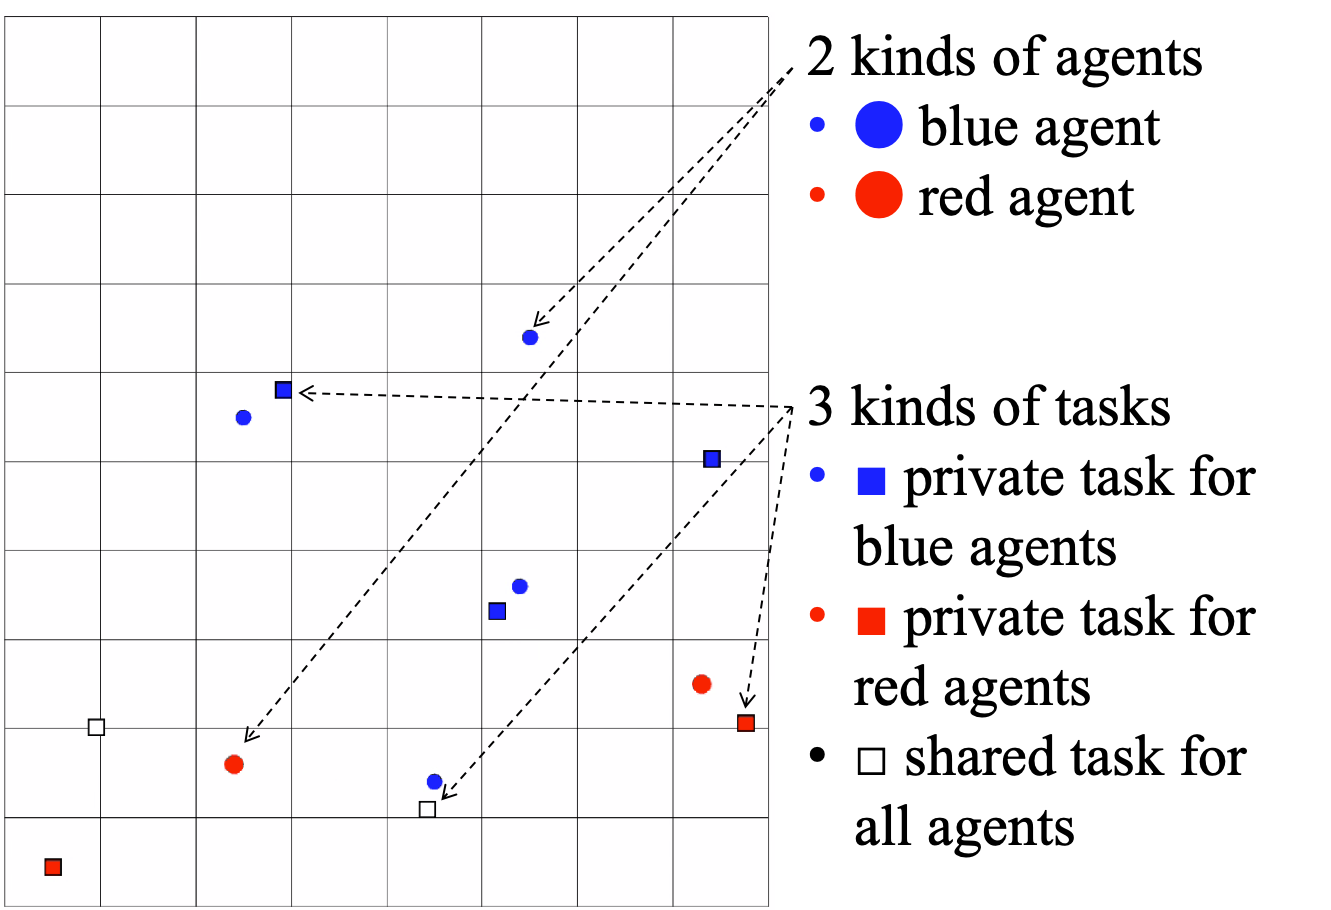
\includegraphics[width=3.4in]{Workspace_intruders_new.png}
    \caption{In this example, the workspace is partitioned into $80$ vertices. There are 2 kinds of heterogeneous agents (blue and red) that have to perform the tasks in the workspace. There are 2 kinds of private tasks (blue and red) for the 2 kinds of agents, and 1 kind of shared tasks (white) that can be done by any agent.}
    \label{fig:workspace}
\end{figure}

Throughout this paper, we refer to the robots as "robots" or "agents" interchangeably. The set of all agents is denoted by $\A$, which is subdivided into $F$ disjoint fleets $\A^1,\ldots, \A^F$, where agents within the same fleet are considered to be of homogeneous capabilities.
\frline{}{Comment on how this captures a number of cases of interest where there is a large population of agents belonging to two-three types, e.g. aerial and ground vehicles, or vehicles equipped with different sensor packets, etc.}
We denote by $a_f=|\A^f|$ the number of agents in a given fleet $f$, and by $\F=\{1,\ldots,F\}$ the set of fleet indices. 

The agents are mobile and transition from one vertex $i\in \V$ to another $j\in \V$ every time step, assuming that $(i,j)\in E$.\footnote{Agents can stay put in vertex $i$ if $(i,i)\in \E$.}
For a given fleet $f\in \F$, the positions of its agents at time $\tau\in [T]$ are specified by $p^f_\tau\in [a_f]^{ |\V|}$, where for a given $i\in \V$, $p^f_\tau[i]$, specifies the number of agents of $\A^f$ located at the vertex. %Agents can move Given that agent $q\in \A$ is located in $i\in \V$ at time step $\tau\in [T-1]$ (i.e., $p^q_\tau[i]=1$), it moves to an adjacent vertex $j\in \E_+(i)$ in the next time step (i.e., $p^q_{\tau+1}[j]==1$), 

\subsection{Shared and Private Task Sets}
The problem consists of allocating agents to tasks which consist of collecting rewards along the time-expanded vertices of $\G$. For now, we assume that the distributions of rewards are known in advance. An extension in which rewards are predicted according to a stochastic process is discussed later on.

There are $F+1$ types of rewards $R^0,R^1,\ldots,R^F$, which determine the values gained by the agents for visiting any given vertex $i\in \V$ at time $\tau\in [T]$.
The type $t\in [F]$ denotes the ability of agents to collect the reward, or to execute a task associated with the reward. Specifically, rewards of type $t=0$ are considered to be \emph{shared}, i.e., can be collected by any robot of any fleet $f\in \F$. In particular, for any $i\in \V, \tau\in [T]$, the system gains the reward $R^0_\tau[i_\tau]$ if $\sum_{f\in \F}p^f_\tau[i]\geq 1$, i.e.,  at least one agent (from any fleet) visits the vertex $i$ at time $\tau$.
In contrast, tasks of type $t \neq 0$ are considered to be \emph{private}, and can only be gained via  agents from the particular fleet $\A^f$ such that $f=t$. That is, when $t\neq 0$ then for any $i\in \V,\tau\in [T]$, the system gains the reward $R^t_\tau[i]$ if $p^t_\tau[i]\geq 1$, i.e.,  at least one agent from $\A^t$ visits the vertex $i$ at time $\tau$. 


\subsection{Problem Formulation}
We are in a position to provide a formal definition of our problem in the form of an integer program. The input to the problem consists of the workspace graph $G$, time horizon $T\in \dN_{>0}$, agent fleets $\A^1,\ldots,\A^F$ with $F\in \dN_{>0}$ with known initial positions $p^f_0[i]$ for all $i\in V$, and potential rewards $R^0,\ldots, R^F$. 

The goal of this work is to obtain a task-allocation scheme, which maximizes the total collected reward. The task-allocation scheme consists of (i) specifying the locations of all agents for every $\tau \in [T]$ and (ii) assigning agents to rewards. We present a formal description of the problem in the form of an integer program in Table~\ref{tbl:heterogeneous} below. 

The scheme is described through two types of decision variables. We use the discrete variable $x^f_\tau[i,j]\in [a_f]$ to denote a transition of agents in $\A^f$ from $i\in \V$ to $j\in \V$, at time $\tau\in [T-1]$, assuming that $(i,j)\in \E$.  
We use the decision variable $y^f_\tau[i]\in \{0,1\}$ to indicate whether an agent from $\A^f$ is assigned to collect the shared reward $R^0_\tau[i]$. 
Similarly, for a given $f\in \F$, the variable $z^f_\tau[i]\in \{0,1\}$ indicates whether an agent in $\A^f$  is assigned to collect the private reward $R^f_\tau[i]$. 

The objective function is given in Equation~\eqref{eq:objective_het} in Table~\ref{tbl:heterogeneous}. Equation~\eqref{eq:flow_conservation} ensures the flow conservation of agents. 
Equations~\eqref{eq:bound_y_1}, \eqref{eq:bound_y_2}, \eqref{eq:bound_z_1}, \eqref{eq:bound_z_2} ensure that an agent is assigned to a task only if it is present in the corresponding vertex.    Equations~\eqref{eq:bound_y_3}, \eqref{eq:bound_z_3} limit the number of agents assigned to every type of task in a given vertex to $1$. 
%\todo{Mention that we wish to solve this problem in a distributed manner.}

\subsection{Predictive Formulation}
We mention that that the above formulation can be easily adapted to the predictive setting. Namely, in this case the precise value of the rewards $R^0,\ldots,R^f$ are only known for the current timestep $\tau=0$, but a stochastic model of the evolution of rewards with respect to time is available in order to predict the rewards' behavior. To exploit the aforementioned deterministic formulation, it is straightforward to show that by plugging into the problem defined in Table~\ref{tbl:heterogeneous} the expected values of the stochastic rewards, the solution would maximize the expected gained reward. This in turn gives rise to a receding-horizon implementation: given the current state of the system (e.g., locations of agents and values of current rewards) we predict the reward values $R^0,\ldots,R^F$ for $T$ time steps into the future, and then compute a plan specified by $x,y,z$. We then execute this plan for the first time step, obtain current values of the reward, and repeat this process all over again. 

We proceed to provide some concrete definitions and an example.
\ksline{I'm not sure how to write formally the definition for the evolving tasks. Can anyone assist?}

To make those definition more concrete, suppose we have two tasks which represent tracking of two distinct objects (one in each task), where the reward for successful tracking are $1, 2$, respectively. Also assume that the objects are confined to a $3\times 3$ grid graph, and that in each time step, each object selects one of its neighbors uniformly at random (and cannot stay in the same vertex). Figure \ref{fig:distribution_and_reward} shows the expected reward $T^t$ for the two task classes (depicted in blue and red respectively) across three time steps.

\begin{figure}[h]
\centering
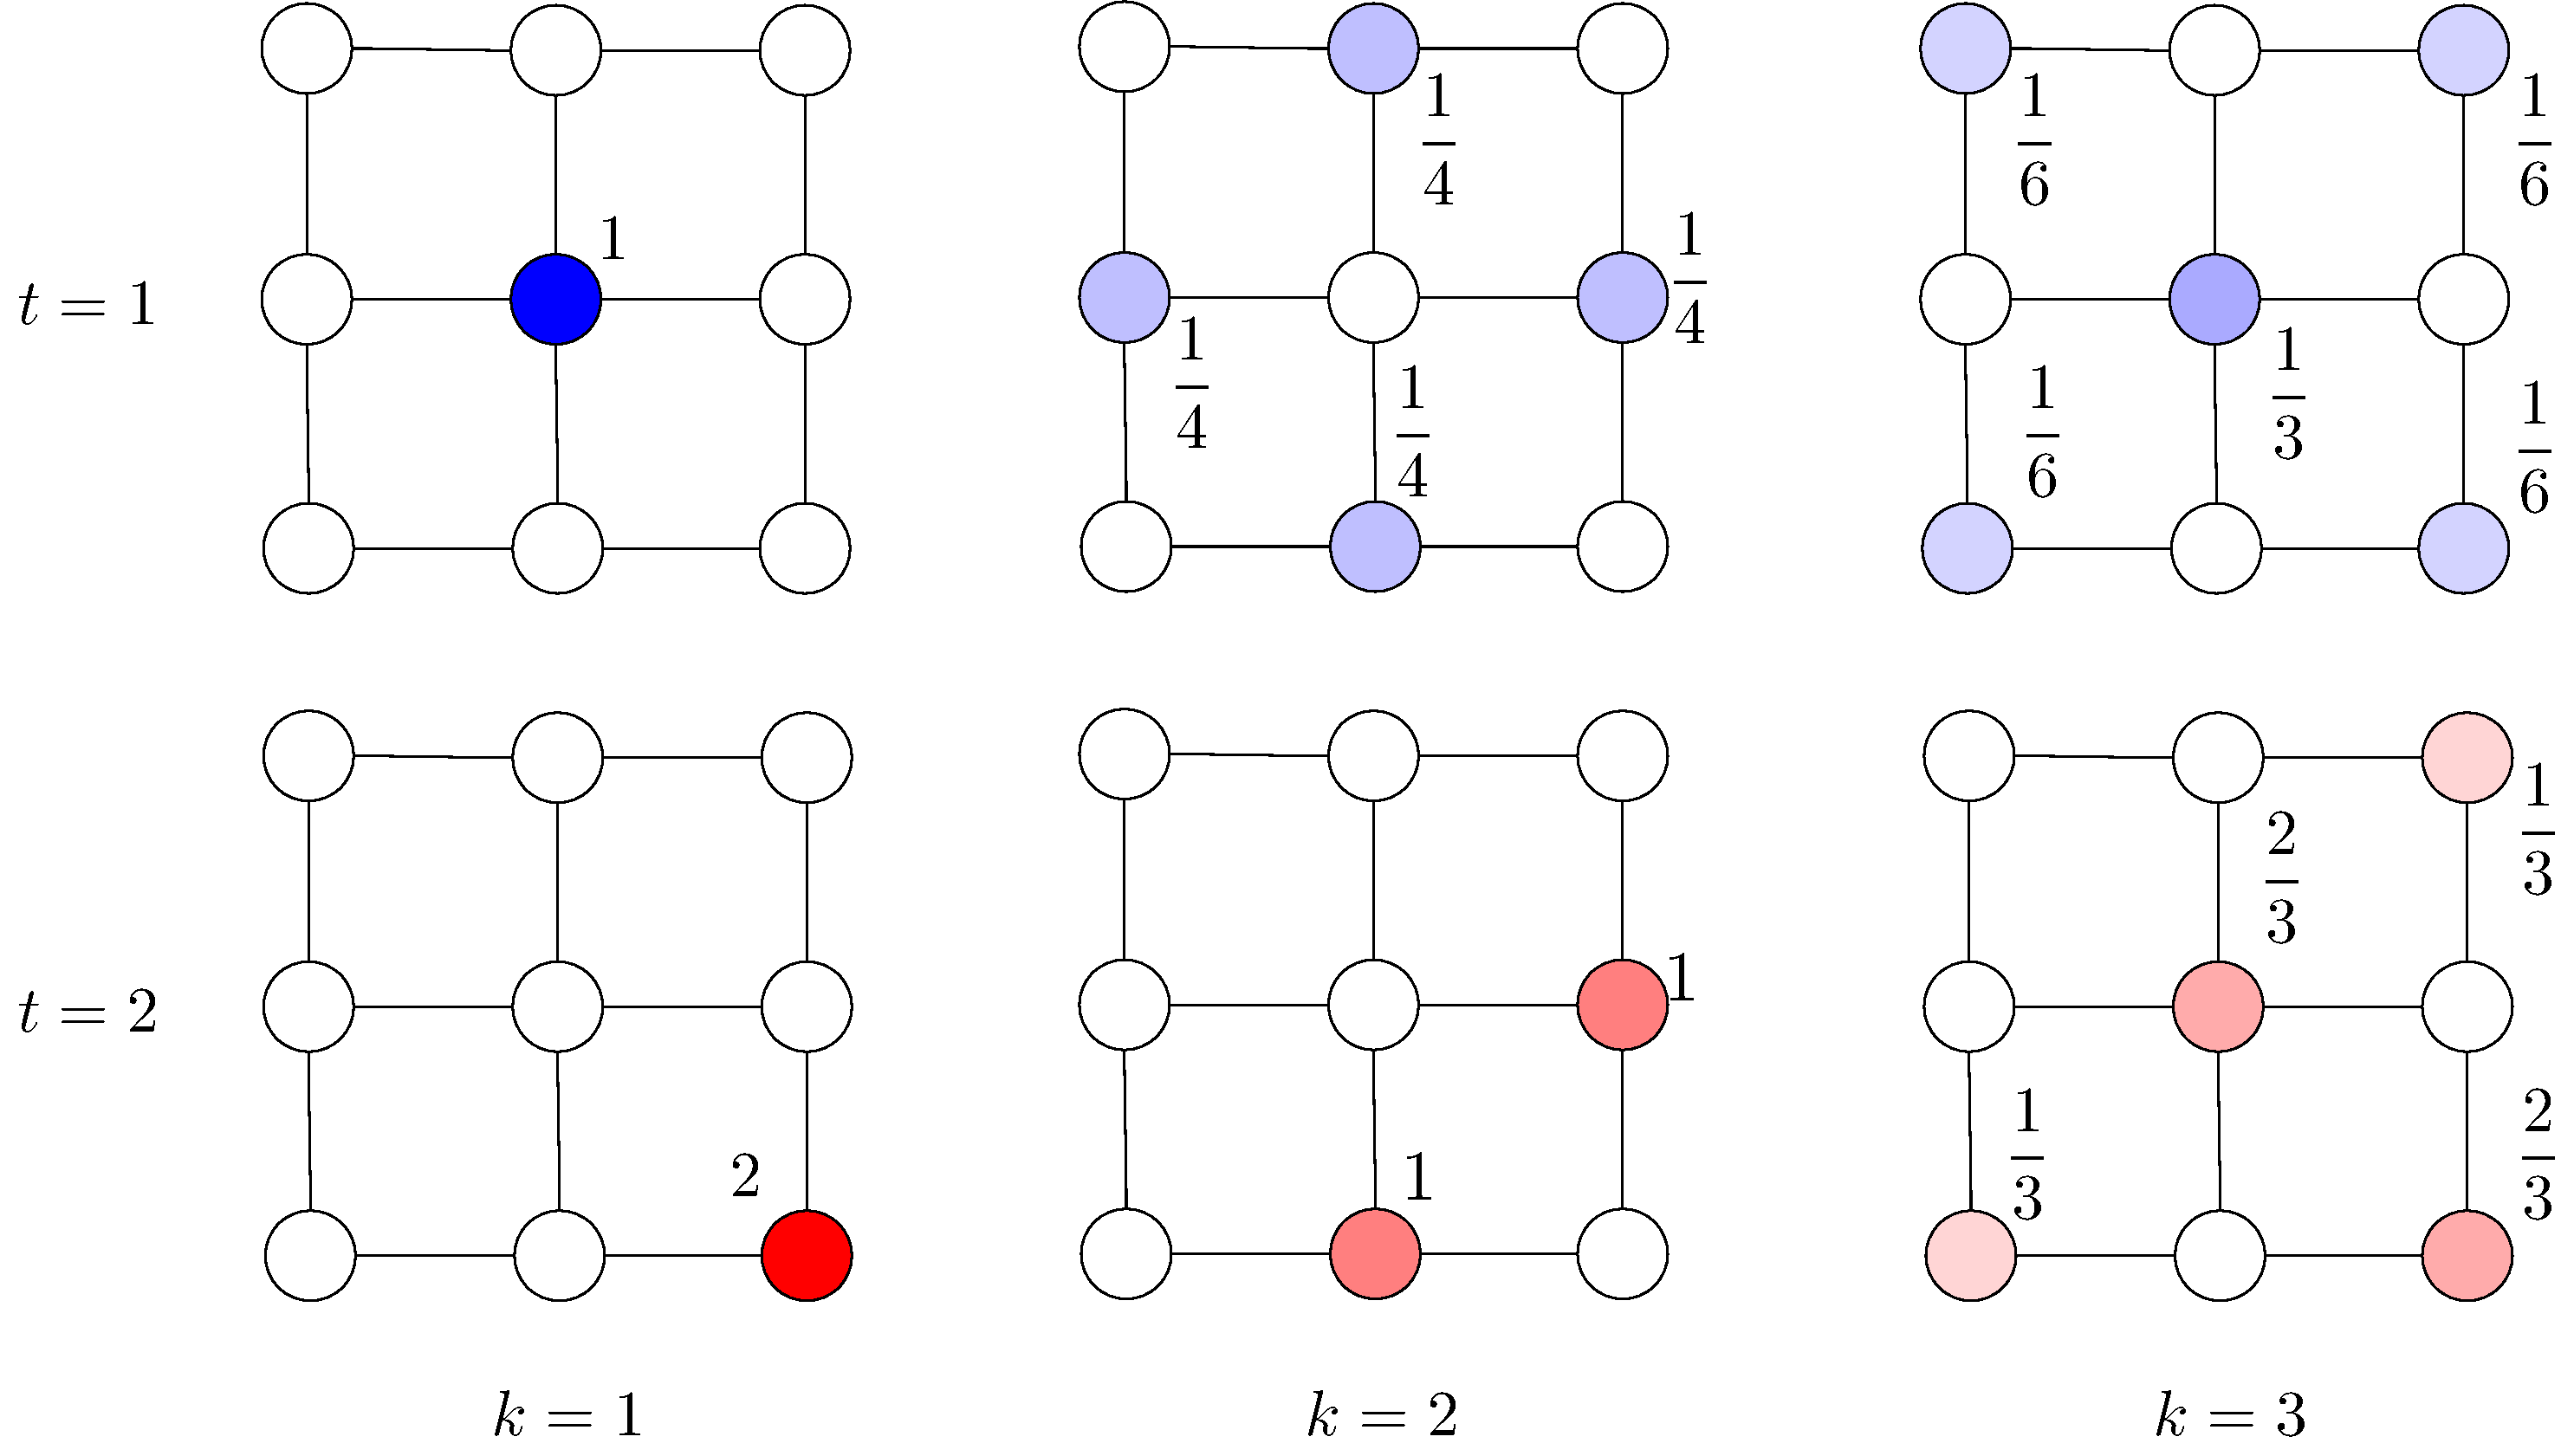
\includegraphics[width=.35\textwidth]{fig/distribution_and_reward.pdf}
\caption{Expected reward for two task classes. The tasks require tracking of an object moving to adjacent cells according to a random walk.}
\label{fig:distribution_and_reward}
\end{figure}

\subsection{Discussion}
\todo{Mention the limitation of our model. Namely that we do not permit settings in which the reward changes based on our actions. }
\todo{Mention that formulation can extend to travel cost.}
We mention that a setting with a similar partition between agents has be explored in~\cite{PrasadETAL18}, albeit for a different problem formulation consisting of computing multiple travelling-salesman routes in an undirected and time-invariant graph. Table~\ref{tbl:problem} is a mixed-integer linear program, and its complexity scales exponentially with the number of variables. %Furthermore, the formulation is centralized, requiring a node to solve the full problem and then communicate to agents their allocations. %In this paper, we propose a distributed approximation algorithm that tackles both these difficulties. 
In the following sections, we develop a centralized approximation algorithm that relies on solving a sequence of homogeneous subproblems. %linear programs, while a distributed implementation is proposed in Section~\ref{sec:distributed_implementation}.

\section{Algorithm for the Homogeneous Case}
In preparation to tackling the heterogeneous problem presented in the previous section, we first consider the simplified homogeneous subcase. Namely, the homogeneous problem consist of a single fleet of homogeneous agents $\A^f$ and a single individual reward set $R^f$. In this section we show that an optimal solution to the homogeneous problem can be found efficiently using an approach for the min-cost flow problem, which will be defined below. An algorithm for solving the homogeneous setting will then be employed in the next section as a subroutine to achieve a polynomial-time approximation for the heterogeneous case.

\begin{table}[!ht]
\label{tbl:homogeneous}
\noindent\fbox{\begin{minipage}[t]{0.48\textwidth - 2\fboxsep - 2\fboxrule}%
Given the graph $\G$, time horizon $T\in \dN_{>0}$, agent fleet $A^f$, initial positions $p_0$, and potential rewards $R^f$,
      \begin{subequations}
        \begin{align}
          \textrm{maximize} \quad  \R^f(x,z):= \sum_{i\in \V} \sum_{\tau\in [T]}  R^f_\tau[i]\cdot z^f_\tau[i], \label{eq:objective_hom}
        \end{align}
\begin{align}
 \textrm{subject to  (\ref{eq:init_position}), (\ref{eq:flow_conservation}), (\ref{eq:bound_z_1}), (\ref{eq:bound_z_2}), (\ref{eq:bound_z_3}), } \text{ with respect to } \A^f. \nonumber 
\end{align}
\end{subequations}
\end{minipage}}
\vspace{5pt}
\caption{Definition of the heterogeneous task-allocation problem.}
\end{table}

For a given reward set $R^f$ and initial positions of $\A^f$ encoded through $0^f$, we denote by  $\H(R^f, p_0^f)$ the homogenenous optimization problem in Table \ref{tbl:homogeneous}.%, and the pair $(x^f,z^f)$ is the optimal solution of this homogeneous problem.
Note that the problem of assigning the set of shared tasks $R^0$ to all the agents $\A$, while ignoring the assignment of private tasks, can be viewed as the homogeneous problem $\H(R^0,p)$.
 
The motivation for considering the homogeneous case is given in the following theorem, which states that an optimal solution to this problem can be obtained in (low-degree) polynomial time.

\begin{theorem}\label{thm:homogeneous}
  For any $f\in \F$, the optimal solution for $\H(R^f, p^f_0)$ (similarly for $\H(R^0,p_0)$) can be computed in 
  $$\O\left(T^2mn\log (Tn)+T^2n^2\log (Tn)\right)$$
  time, where $m=|\E|,n=|V|$. 
\end{theorem}
\begin{proof}
  In this proof we show that the homogeneous problem can be transformed into a min-cost flow (MCF) problem~\cite{Williamson2019}, for which an optimal solution can be efficiently found. In the remainder of this proof we define the ingredients for MCF, then provide a formal definition of the problem, and then discuss its complexity.

MCF is defined for a directed graph whose edges are weighted and have capacity constraints. For a given instance $\H(R^f,p^f)$ we define the graph $\dG=(\dV,\dE)$, where
$$\dV=\{s,g\}\cup\{v^i_\tau,w^i_\tau|i\in \V,\tau\in T\}.$$
That is, the vertex set consists of the vertices $s$ and $g$, which will be used as the source and sink of the flow, respectively, as well as two copies $v^i_\tau,w^i_\tau$ of every vertex $v\in \V$ for each time step $\tau\in T$. 

The edge set is defined for several subsets $\dE=E_{s}\cup E_t\cup E_0\cup E_{R}\cup E_1$, where
\begin{align*}
  E_s&=\{(s,v^i_0)|\exists q\in \A^f p^q_0[i]\neq 0\},\\
  E_g&=\{(w^i_T,g)|i\in \V\},\\
  E_0&=\{(v^i_\tau,w^i_\tau)|i\in \V, \tau\in [T]\},\\
  E_{R}&=\{(v^i_\tau,w^i_\tau)|i\in \V, \tau\in [T],R^f_\tau[i]\neq 0\},\\
  E_{\E}&=\{(w^i_\tau,v^j_{\tau+1})|(i,j)\in \E, \tau\in [T-1]\}.  
\end{align*}
Namely, edges in $E_s$ connect the source vertex $s$ to all the vertices which function as start positions for the agents. Edges in $E_g$ connect all the vertices in the final time step $T$ to the sink node $g$. Edges in $E_0$ connect between every two copies $v^i_\tau,w^i_\tau$ of a vertex $i\in V$ for a given time step $\tau$. Agents traversing the latter set of edges will receive no reward. On the other hand, every edge $(v^i_\tau,w^i_\tau)\in E_R$ will be used to represent the collection of the reward $R^f_\tau[i]$ by the agent traversing this edge. Edges in $E_{\E}$ simulate the traversal of agents along the edges of $\E$ between one time step to the next. 

Next, we assign costs $c$ for the edges in $\dE$. In particular, for any $e\in \dE\setminus E_R$ we set $c_e:=0$. For a given $e'\in(v^i_\tau,w^i_\tau)\in E_R$ we set $c_{e'}:=-R^f_\tau[i]$. The final ingredient to the MCF problem is edge capacities $u$. For any $e\in E_g\cup E_0\cup E_\E$ we set infinite capacity $u_e:=\infty$. To ensure that the correct number of agents will arrive to the starting positions, we specify for a given $e'=(s,v_0^i)\in E_s$ the capacity $u_{c'}:=\sum_{q\in \A^f}p_0^q[i]$. Finally, to ensure that every reward will be collected by at most one agent, we specify $u_{e''}:=1$ for any $e''\in E_R$. 

We are ready to provide the corresponding formulation of MCF. The goal is to assign flow values $h_e\in [0,\infty)$, which represent the number of agents traversing $e$, to all edges $e\in \dE$ in order to minimize the expression $\sum_{e\in \dE}h_e c_e$ under the constraints 
\begin{subequations}
\begin{align}
 h_{e}&\in [0,u_e],  \forall e\in \dE,\label{eq:mcf:bound}\\
 \sum_{e\in E_s}h_{e}& =|\A^f|, \label{eq:mcf:source}\\
  \sum_{e\in E_g}h_{e}& =|\A^f|, \label{eq:mcf:sink}\\
  \sum_{v'\in \dE^+(v)}h_{vv'}-\sum_{v'\in \dE^-(v)}h_{v'v}&= 0, \forall v\in \dV\setminus \{s,g\}.\label{eq:mcf:else}
\end{align}
\end{subequations}
Constraint \eqref{eq:mcf:bound} ensures that capacities are maintained; \eqref{eq:mcf:source} ensures that all the agents will leave the source; \eqref{eq:mcf:sink} ensures that all agents will end up at the sink vertex\footnote{For our specific graph structure $\dG$, and considering the constraint \eqref{eq:mcf:else}, the constraint \eqref{eq:mcf:sink} is redundant. We leave it for clarity and completeness.}; the final constraint ensures equality between the number of agents leaving and entering a vertex $v\in \dV\setminus \{s,g\}$.

By definition of $\dG,c,u$ its clear that the above MCF formulation is equivalent to the homogeneous problem, with one slight change. Namely, MCF permits fractional assignments to $h$, whereas the values of $x,z$ are integral. If all edge capacities are integral (which is the case in our setting), the linear relaxation of MCF enjoys a totally-unimodular constraint matrix form~\cite{AhujaETAL93}. Hence, the fractional solution will necessarily have an integer optimal solution. 

We note that the above MCF problem can be solved in $\O((M'+N)\log N(M+N\log N))$ time using Orlin's MCF algorthim~\cite{Orlin93,Williamson2019}, where $M=|\dE|=\O(Tm)$, $N=|\dV|=\O(Tn)$, and $M'$ is the number of $\dG$ edges whose capacity is finite. In our case $M'=\O(Tn)$, which implies that the total time complexity of MCF is $\O(T^2mn\log n+T^2n^2\log^2n)$. 

%Finally, we address (ii), by showing that given a MCF solution represented by $h$, we can transform it into assignments of $x,z$ for all agents $q\in \A^f$ in time $\O(Ta_f)$, where $a_f=|\A^f|$. Our goal is to extract using $h$ a collection of $|\A^f|$ edge-disjoint paths from $s$ to $g$ (with respect to $\dG$) such that every edge $e\in \dE$ appears in exactly $h_e$ paths.  

%Denote by $\dG_h$ the subgraph of $\dG$ induced by $h$, such that $e\in \dG_h$ for $e\in \dG$ if $h_e>0$. Note that the latter can be constructed in $\O(\dE)$ time. In the following discussion we shall assume that $\dG_h$ is represented by a directed adjacency list. Given $\dG_h$ we find a path in the graph that connects $s$ to $g$ by beginning with $s$, selecting its first neighbor $v\in \dG_h$ in the adjacency list, and repeating this process until $g$ is reached. Denote the collection of edge along this route as $P$. (Notice that this process takes $\O(T)$ time, which corresponds to $|P|$.) Using this route $P$ we assign the values of $x^q,z^q$ for the first agent $q\in \A^f$. Next, we update $h$ by assigning $h_e:=h_e-1$ for every $e\in P$, and update $\dG_h$ by eliminating edges for which $h_e=0$. Given the updated $dG_h$, we find a new route for the next agent, and repeat this process for a total of $|\A^f|$ repetitions, where each one requires $\O(T)$ time in total. 
%
%To conclude, we showed how to compute a solution for $\H(R^f,\A^f)$, by computing a MCF formulation of the problem in time $\O(T^2mn\log n+T^2n^2\log^2n)$, and then transformed into assignments $x$ and $z$ in time $\O(Tm+Ta_f)$. The total running time is 
%$$\O(T^2mn\log n+T^2n^2\log^2n+Ta_f).\qedhere$$
\end{proof}

\section{Algorithm for the Heterogeneous Case}\label{sec:centralized}
In this section we present an efficient algorithm to tackle the task-allocation problem described in Table~\ref{tbl:heterogeneous}. %For now, we consider a centralized version of it; a distributed implementation is provided in Section \ref{sec:distributed_implementation}. 
Recall that we wish to find an assignment $x,y,z$ such that the expression $\R(x,y,z)$ is minimized, where for a given $f\in \F$, $\tau \in [T]$, $j\in V$, $x_{\tau}^f[i,j]$ represents the transitions of the agents in $\A^f$, and $y_{\tau}^f[i]$, $z_{\tau}^f[i]$ indicate whether it is assigned in vertex $i$ to execute $R_{\tau}^0[i]$ and $R_{\tau}^f[i]$ respectively. 

For a given $f\in \F$, denote by $x^f$ the corresponding values of the $x$ assignment for agents of fleet $f$, i.e., $x^f=\{x^f_{\tau}\}_{\tau\in [T-1]}$ for $\tau \in [T]$. The sets $y^f,z^f$ are similarly defined. 

\subsection{Algorithm}
We present the private-first-shared-first (\alg) algorithm for heterogeneous task allocation (see  Algorithm~\ref{alg:main}). It accepts as input the specification of the agents and the entire reward set $\dR=\{R^0,R^1,\ldots,R^F\}$. It then obtains two candidate solutions $(x,y,z),(x',y',z')$ and returns the one that yields the larger reward of the two. 

\begin{algorithm}[!ht]
  $(x,y,z)\gets \private(\dR,p_0)$\;
  $(x',y',z')\gets \shared(\dR,p_0)$\;
  \If {$\R(x,y,z)>\R(x',y',z')$}{
    \Return $(x,y,z)$\;
    }
  \Return $(x',y',z')$\;
  \caption{\alg$(\dR,p_0)$}
  \label{alg:main}
\end{algorithm} 

The subroutine \private (Algorithm~\ref{alg:private}) prioritizes the assignment of private rewards over shared rewards. This is achieved by assigning to each fleet $f\in \F$ a new reward set $\hat{R}^f$ which consists of the combination of its private reward set $R^f$ and the shared reward set $R^0$, where the latter's rewards are rescaled by $F^{-1}$ with $F=|\F|$. That is, $\hat{R}^f_\tau[j]={R}^f_\tau[j]+ {R}^0_\tau[j]\cdot F^{-1}$. An assignment over $\hat{R}^f$ for every $f\in \F$ is then obtained. Note that $z^f$ implicitly encodes both an assignment to a private reward, as well as the shared one. That is, an agent assigned to perform a reward $\hat{R}^f_\tau[j]$ can be interpreted as being assigned to both $R^f_\tau[j]$ and $R^0_\tau[j]$.
In lines 4-8 the solutions of the individual fleets are combined to eliminate cases where several agents (from different fleets) are assigned to the same shared reward. To do so, for a given $\tau,j$, we go iteratively over all fleets $f\in \F$ and set $y^f_\tau[j]=1$ for the first agent we encounter that is assigned to a shared reward in the corresponding vertex. 

\begin{algorithm}[!ht]
  $\hat{R}^f\gets R^f+R^0\cdot F^{-1}, \forall f\in \F$\;
  $(x^f,z^f)\gets \H(\hat{R}^f,p_0^f), \forall f\in \F$\;
  $x\gets \{x^f\}_{f\in \F},z\gets\{z^f\}_{f\in \F}$\;
  $y\gets \{\{0\}_{q\in \A}\}_{\tau \in [T]}$\;
  \For{$\tau\in [T], j\in \V$}{
    \For{$f\in \F$}{
        \If{$z_\tau^f[j]==1$}{
            $y_\tau^f[j]\gets 1$\;
            break \;
            }
        }
    }
  \Return $(x,y,z)$\;
  \caption{$\private(\dR,p_0)$}
  \label{alg:private}
\end{algorithm} 

The \shared subroutine (Algorithm~\ref{alg:shared}) prioritizes the assignment of shared rewards, by first computing the an assignment for all the agents $\A$ to the shared reward set $R^0$, to maximize the total reward. This is achieved by calling $\H(R^0,p_0)$.  It then generates an updated reward set $\bar{R}^f$ for every fleet $f\in \F$, where the value of a reward $\bar{R}^f_\tau [j]$ is equal to $R^f_\tau [j]$ in case that $R^0_\tau[j]$ was not assigned to $f$, and otherwise equal to $R^f_\tau [j]+R^0_\tau[j]$. Next, for every fleet $f$ the private assignment $(x^f,z^f)$ over $\bar{R}^f$ is computed. Observe that $z$ represents simultaneously assignments for shared and private rewards.

\begin{algorithm}[!ht]
    $(\bar{x},\bar{y})\gets \H(R^0,p_0)$\; 
    %$\bar{R}^f\gets R^f, \forall f\in \F$\;
    \For{$f\in \F, \tau\in [T], j\in \V$}{
        $\bar{R}^f_\tau[j]\gets {R}^f_\tau[j]+R^0_\tau[j]\cdot\bar{y}_\tau^f[j]$\;
    }
  $(x^f,z^f)\gets \H(\bar{R}^f,p_0), \forall f\in \F$\;
  $x\gets \{x^f\}_{f\in \F},z\gets\{z^f\}_{f\in \F}$\;
  \Return $(x,z,z)$\;
  \caption{$\shared(\dR,p_0)$}
  \label{alg:shared}
\end{algorithm} 

\subsection{Analysis}
In this section, we show that, for a given number of fleets $F$, the PFSF algorithm is guaranteed to achieve a solution within a constant factor of the optimum. Then we provide a computational analysis of the approach.

\todo{Define $S^*,P^*$ for the optimal value for the shared and private rewards. Consider two cases for the shared reward. Include in the main theorem a consideratin for the case that $P^*\neq 0$, in which case there exists $\Delta$ such that $S^*:=\Delta P^*$.}

Let $(x,y,z)$ be an assignment returned by \alg. With a slight abuse of notation, we use $\R(x^f,y^f,z^f)$ to represent the reward obtained by agents of fleet $f\in \F$ (where assignments values of agents in other fleets are set to $0$). Similarly, $\R(x,y,\bm{0}), \R(x,\bm{0},z)$ represent the reward gained from shared rewards and private rewards, respectively, where $\bm{0}$ represents the zero vector (whose dimension will be clear from context). 

Let $(X,Y,Z)$ be the optimal assignment. It will be convenient to define
$\textsc{opt}:=\R(X,Y,Z)=S^*+P^*$, where 
\begin{align*}S^*&:=\R(X,Y,\bm{0}), \\ P^*&:=\R(X,\bm{0},Z)=\sum_{f\in \F}\R({X}^f,\bm{0},{Z}^f).\end{align*}
We are ready to state our main theoretical contribution:

\begin{theorem}[Approximation factor of PFSF]\label{thm:main}
  Let $(x,y,z)$ be the solution returned by \alg. Then $\R(x,y,z)\geq \textsc{opt}\cdot \frac{F}{2F-1}$. 
\end{theorem}

Before proceeding to the proof of the main theorem, we establish two intermediate results, concerning the guarantees of \private and \shared, when considered separately. In particular, we show that each of the subroutines provide complementary approximations with respect to $S^*$ and $P^*$, and PFSF enjoys the best of both worlds. See illustration in Figure~\ref{fig:approximation}

\begin{figure}[!ht]
    \centering
    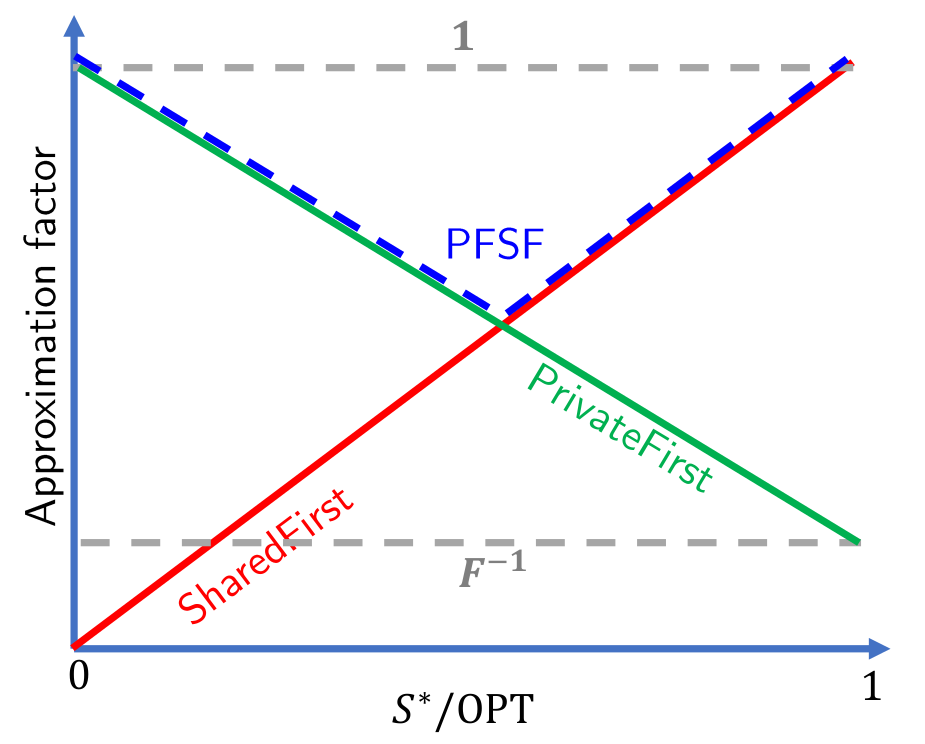
\includegraphics[width=2.5in]{approximation.png}
    \caption{Visualization of the approximation factors (y-axis) achieved by PFSF (dashed blue curve), \private (green curve), \shared (red curve), as a function of the ratio between $S^*$ and OPT.}
    \label{fig:approximation}
\end{figure}


\begin{lemma}Approximation factor of \private]\label{lem:private}
  Let $(x,y,z)$ be the solution returned by \private. Then $\R(x,y,z)\geq \Delta\cdot  S^*\cdot F^{-1}+P^*$.
\end{lemma}
\begin{proof}
  Fix $f\in \F$ and note that
  \[\R(x^f,y^f,z^f) \geq \R\left({X}^f,\bm{0},{Z}^f\right)+F^{-1}\cdot \R(X^f,Y^f,\bm{0}),\]
  since \private could choose to assign $(x^f,z^f)=(X,Y+Z)$ (line~2), which would yield the desired result. Hence,
\begin{align*}
  \R(x,y,z)&=\sum_{f\in \F}\R(x^f,y^f,z^f)\\ & \geq  \sum_{f\in \F}\R\left({X}^f,\bm{0},{Z}^f\right)+F^{-1}\sum_{f\in \F}\R (X^f,Y^f,\bm{0}) \\ 
& =P^* + F^{-1}\cdot S^*.
\end{align*}
\end{proof}

\begin{lemma}[Approximation factor of \shared]\label{lem:shared}
  Let $(x,y,z)$ be the solution returned by \shared. Then $\R(x,y,z)\geq S^*$.
\end{lemma}
\begin{proof}
  The proof is straightforward, as it must hold that $\R(\bar{x},\bar{y},\bm{0})\geq \R(X,Y,\bm{0})$, where $\bar{x},\bar{y}$ are as defined in line~1 of \shared.
\end{proof}

We are ready for the main proof:
\begin{proof}[Proof of Theorem~\ref{thm:main}]
Due to Lemma~\ref{lem:private}, and Lemma~\ref{lem:shared}, it is clear that \alg obtains a solution $(x,y,z)$ with reward at least $\max\left\{P^*+F^{-1}\cdot S^*,S^*\right\}$. Next, observe that if either of $S^*$ or $P^*$ is zero, the PFSF would necessarily return the optimal solution. Now, assume that $S^*$ and $P^*$ are strictly positive, and hence there exists $\Delta>0$ such that $P^*=\Delta S^*$. 
We have that 
\begin{align*}
    \frac{\R(x,y,z)}{\R(X,Y,Z)} & \geq \frac{\max\left\{\Delta\cdot S^*+F^{-1}\cdot S^*,S^*\right\}}{\Delta S^*+S^*} \\ & 
    = \max\left\{\frac{\Delta+F^{-1}}{\Delta +1},\frac{1}{\Delta+1}\right\}\\ 
    & \geq 
    \max\left\{\frac{\frac{F-1}{F}+F^{-1}}{\frac{F-1}{F} +1},\frac{1}{\frac{F-1}{F}+1}\right\}\\ & = \frac{F}{2F-1},
\end{align*}
where we used the fact that $\argmin_{\Delta>0}\max\left\{\frac{\Delta+F^{-1}}{\Delta +1},\frac{1}{\Delta+1}\right\}=(F-1)/F.$
\end{proof}

We conclude this section with a computational analysis of the overall approach. 

\begin{corollary}
  \alg can be implemented in $\O(FT^2mn\log n+FT^2n^2\log^2n)$ time.
\end{corollary}
\begin{proof}
  This result directly follows from Theorem~\ref{thm:homogeneous}, as we perform $2F+1$ computations of $\H$, where each computation is a bottleneck for both \private and \shared. \ksline{}{Consider elaborating how the flow decomposition is achieved.}
\end{proof}

\begin{comment}
    \subsection{Discussion}
    A few comments are in order.
    \frline{- Is the approximation factor good? We get at least 1/2, which is surprisingly good. Plus, in simulations we show that in practical applications we do much better than that...or something.
    - The assumption that we know the distribution of tasks is strong. Future work will look at the setting where this distribution is learned on the fly, which introduces an interesting exploration/exploitation problem.
    - }{TODO}
\end{comment}

\begin{table*}[!ht]
\noindent\fbox{\begin{minipage}[t]{1\textwidth - 2\fboxsep - 2\fboxrule}%
\begin{subequations}
\begin{align}
\underset{\begin{array}{ll}
x_{\tau}^{q}[i,j] & \forall (i,j) \in \E, \thinspace  \tau \in \K_k, \\
z_\tau^q[j] & \forall j\in \V,  \thinspace \forall \tau \in \K_k \cup \{k + K_{\textrm{hor}}+1 \}, 
\end{array}}{\textrm{maximize}} \left( \Ex_{\dT\in \Lambda_k} \left[\bar{\R}^f(x^q,z^q)\right] \right) \textcolor{red}{\textbf{--}} \left( \sum_{\tau \in \K_k \cup \{k + K_{\textrm{hor}}+1 \} } \sum_{j \in \V} \lambda_{\tau}[j]   \left(  z_{\tau}^q[j] - \frac{1}{|\A^f|}  \right) \right) \label{eq:objective_function_new_homo_decomposed} 
\end{align}
\begin{align}
\textup{where }\quad \bar{\R}^f(x^q,z^q):= \left( \sum_{\tau \in \K_k \cup \{k + K_{\textrm{hor}}+1 \} } \sum_{j \in \V}  \left( T_\tau^f[j]\cdot z_{\tau}^q[j] \right) \right)   , \label{eq:objective_f_homo_decomposed}
\end{align}
\begin{align}
\textrm{subject to} \nonumber \\
0 \leq x_{\tau}^q[i,j] & \leq 1 \thinspace, & & \forall (i,j) \in \E, & & \forall \tau \in \K_k, \label{eq:init_x_relaxed_lower_decomposed} \\
% x_{\tau}^q[i,j] & \leq 1 \thinspace, & & \forall (i,j) \in \E, & & \forall \tau \in \K_k, \label{eq:init_x_relaxed_upper_decomposed} \\
% \sum_{j \in \N(i)} x_\tau^q[i,j] & = p_{k}^q[i] \thinspace, & &  \forall i \in \V, \label{eq:init_position_relaxed_decomposed} \\  % Replace by 1d
% \sum_{i \in \N(j)} x_{\tau}^q[i,j] & = \sum_{\ell \in \N(j)} x_{\tau + 1}^q[j,\ell] \thinspace, & & \forall j \in \V, & & \forall \tau \in \{k, \ldots, k + K_{\textrm{hor}}-1 \} , \label{eq:flow_conservation_relaxed_decomposed} \\ % Replace by 1e
0 \leq z_{\tau}^q[i] & \leq 1 \thinspace, & & \forall i \in \V, & & \forall \tau \in \K_k \cup \{k + K_{\textrm{hor}}+1 \} , \label{eq:init_z_relaxed_lower_decomposed} \\
% z_{\tau}^q[i] & \leq 1 \thinspace, & & \forall i \in \V, & & \forall \tau \in \K_k \cup \{k + K_{\textrm{hor}}+1 \} , \label{eq:init_z_relaxed_upper_decomposed} \\
% z_{\tau}^q[i] & \leq  \sum_{j \in \N(i)} x_{\tau}^q[i,j] \thinspace, & & \forall i \in \V, & & \forall \tau \in \K_k , \label{eq:bound_z_1_relaxed_decomposed} \\ % Replace by 1k
% z_{\tau+1}^q[j] & \leq   \sum_{i \in \N(j)} x_{\tau}^q[i,j] \thinspace, & & \forall j \in \V, & & \tau = k + K_{\textrm{hor}},  \label{eq:bound_z_2_relaxed_decomposed}  \\ % Replace by 1l
(\ref{eq:init_position}), (\ref{eq:flow_conservation}), (\ref{eq:bound_z_1}), \textrm{ and } (\ref{eq:bound_z_2}) & & & \textrm{ for agent } q \textrm{ only } \nonumber
%\sum_{q\in\A^f} z_{\tau}^q[i] & \leq 1 , && \forall i\in \V, & & \forall f \in \F , & & \forall \tau\in \K_k \cup \{k + K_{\textrm{hor}}+1\},\label{eq:bound_z_3}
\end{align}
\end{subequations}
    \end{minipage}}
\vspace{5pt}
\caption{Decomposition of the relaxed formulation of the homogeneous task-allocation problem $\H(T^f, \A^f)$ to be solved by agent $q \in \A^f$}
\label{tbl:problem_homo_relaxed_decomposed}
\end{table*}

\section{Experiments}\label{sec:experiments}
In this section we validate our theoretical results from the previous section through simulation experiments. In particular, we demonstrate that our PFSF algorithm  scales well and finds a near-optimal solutions fairly quickly on commodity hardware. Moreover, we show that our approach is faster than a MILP-based approach by several order of magnitude, and we observe that the approximation factors that we achieve are typically larger than the worst-case bound of $\frac{F}{2F-1}$. Additionally, in accordance with the complexity analysis, we observed experimentally that the running time of PFSF is not affected by number of agents within each fleet (as opposed to the number of fleets).

\subsection{Implementation Details}
All results were obtained using a commodity laptop equipped with 2.80GHz $\times$ 4 core i7-7600U CPU, and 16GB of RAM, running 64bit Ubuntu 18.04 OS. We implemented the PFSF algorithm in \cpp, where we used the \texttt{Lemon Graph Library} for the implementation of min-cost flow~\cite{Lemon}. To the best of our knowledge, this library provides the fastest implementation of min-cost flow algorithms~\cite{Kovacs15} (we mention that we used the network-simplex algorithm, which turned to be the fastest in our experiments). We compared our approach with a MILP-based solution using CPLEX~\cite{Cplex}.

\newcolumntype{L}{>{\centering\arraybackslash}m{1cm}}
\begin{table*}[]
\centering
\begin{tabular}{Lc||c|c|c|c|c|c|c|}
\cline{3-9}
                                           &      & \multicolumn{7}{c|}{fleets}    \\ \hline
\multicolumn{1}{|L||}{time horizon}         & criterion & 2 & 4 & 8 & 16 & 32 & 64 & 128 \\ \hline \hline
\multicolumn{1}{|c||}{\multirow{3}{*}{2}}   & MILP & 0.00 & 0.01 & 0.01 & 0.03 & 0.07 & 0.16 & 0.36 \\ \cline{2-9} 
\multicolumn{1}{|c||}{}                     & PFSF & 0.01 & 0.01 & 0.02 & 0.03 & 0.06 & 0.12 & 0.26   \\ \cline{2-9} 
\multicolumn{1}{|c||}{}                     & APX  & 1.00 & 1.00 & 0.93 & 0.86 & 0.64 & 0.75 & 0.75   \\ \hline  \hline
\multicolumn{1}{|c||}{\multirow{3}{*}{4}}   & MILP &  0.02 & 0.04 & 0.07 & 0.16 & 0.39 & 0.90 & 1.77  \\ \cline{2-9} 
\multicolumn{1}{|c||}{}                     & PFSF & 0.01 & 0.03 & 0.05 & 0.09 & 0.17 & 0.35 & 0.67   \\ \cline{2-9} 
\multicolumn{1}{|c||}{}                     & APX  &  1.00 & 0.97 & 0.87 & 0.86 & 0.77 & 0.74 & 0.85    \\ \hline  \hline
\multicolumn{1}{|c||}{\multirow{3}{*}{8}}   & MILP &   0.11 & 0.26 & 0.58 & 1.39 & 3.62 & 12 & 21  \\ \cline{2-9} 
\multicolumn{1}{|c||}{}                     & PFSF &  0.04 & 0.07 & 0.13 & 0.25 & 0.46 & 0.94 & 1.85   \\ \cline{2-9} 
\multicolumn{1}{|c||}{}                     & APX  &  0.96 & 0.92 & 0.82 & 0.80 & 0.84 & 0.88 & 0.94     \\ \hline  \hline
\multicolumn{1}{|c||}{\multirow{3}{*}{16}}  & MILP &  0.45 & 1.40 & 3.78 & 20 & 93 & 453 & DNF   \\ \cline{2-9} 
\multicolumn{1}{|c||}{}                     & PFSF &  0.10 & 0.19 & 0.36 & 0.67 & 1.27 & 2.54 & 5.92   \\ \cline{2-9} 
\multicolumn{1}{|c||}{}                     & APX  & 0.96 & 0.93 & 0.88 & 0.92 & 0.89 & 0.95 &     \\ \hline  \hline
\multicolumn{1}{|c||}{\multirow{3}{*}{32}}  & MILP &  1.5 & 5.6 & 20 & 284 & 567 & DNF & DNF \\ \cline{2-9} 
\multicolumn{1}{|c||}{}                     & PFSF &  0.29 & 0.52 & 1.00 & 1.87 & 3.76 & 7.11 & 16  \\ \cline{2-9} 
\multicolumn{1}{|c||}{}                     & APX  &  0.94 & 0.89 & 0.82 & 0.88 & 0.94 &  &   \\ \hline \hline
\multicolumn{1}{|c||}{\multirow{3}{*}{64}}  & MILP &  4.78 & 21 & 203 & DNF & DNF & DNF & DNF  \\ \cline{2-9} 
\multicolumn{1}{|c||}{}                     & PFSF &  0.84 & 1.50 & 2.78 & 5.22 & 12 & 20 & 43 \\ \cline{2-9} 
\multicolumn{1}{|c||}{}                     & APX  &  0.97 & 0.91 & 0.92 &  &  &  &      \\ \hline  \hline
\multicolumn{1}{|c||}{\multirow{3}{*}{128}} & MILP & 14.20 & DNF & DNF & DNF & DNF & DNF & DNF    \\ \cline{2-9} 
\multicolumn{1}{|c||}{}                     & PFSF &  2.48 & 4.85 & 8.25 & 17 & 31 & 59 & 115  \\ \cline{2-9} 
\multicolumn{1}{|c||}{}                     & APX  &  0.96 &  &  &  &  &  &   \\ \hline  
\end{tabular}
\end{table*}

\begin{table}[]
\begin{tabular}{c|c|c|c|c|c|c|c|}
\cline{2-8}
                                   & \multicolumn{7}{c|}{fleets}    \\ \hline
\multicolumn{1}{|L||}{time horizon} & 2 & 4 & 8 & 16 & 32 & 64 & 128 \\ \hline \hline
\multicolumn{1}{|c||}{2}            & 0.1 & 0.2 & 0.4 & 0.8 & 1.4 & 4.8 & 7.3  \\ \hline
\multicolumn{1}{|c||}{4}            & 0.3 & 0.6 & 1.1 & 2.2 & 4.2 & 13 & 19  \\ \hline
\multicolumn{1}{|c||}{8}            &  1.0 & 1.6 & 3.2 & 6.6 & 12 & 38 & 55  \\ \hline
\multicolumn{1}{|c||}{16}           &  3 & 5 & 9 & 19 & 35 & 118 & 214   \\ \hline
\multicolumn{1}{|c||}{32}           &   9 & 14 & 29 & 59 & 132 & 214 & 414  \\ \hline
\multicolumn{1}{|c||}{64}           &   31 & 48 & 100 & 189 & 375 & 700 & 1423  \\ \hline
\multicolumn{1}{|c||}{128}          &  74 & 154 & 299 & 518 & 994 & 2040 & 4055   \\ \hline
\end{tabular}
\end{table}

\section{Extensions}\label{sec:extensions}
Future tasks are \emph{not} known in advance---however, we assume that outstanding tasks (that is, tasks associated with the current time) are known, and that  a stochastic model of the evolution of tasks with respect to time is available. \frline{The extension to the case where such a model is learned online is an interesting direction for future research.}{Move to discussion}
 
% denote as $\vec{\tau}=\{\tau: (\text{True}, \text{False}) \forall \tau\}$ a Boolean map where $\vec{\tau}_k[\tau]$ is true iff task $\tau$ is performed.
\ksline{Rigorously, denote as $\vec{\tau}_k=\{\tau: (\text{True}, \text{False}) \forall \tau: k_\tau = k\}$ the Boolean map that indicates whether tasks occurring at time $k$ are performed.}{I don't follow this definition. In particular, what is the dimension of $\vec{\tau}_k$, and what do we mean by indicating whether they are performed?}
 
%The probability of occurrence of all tasks associated with time $k$ is denoted as the function $\Lambda_k: \vec{\tau}[k] \mapsto [0, 1]$.
We assume that (i) $\dP(\vec{\tau}_{k+1} | \vec{\tau}_k)$ is known and (ii), at time $k$, $\vec{\tau}_k$ is revealed.
Note that tasks occurring at the same time step can be correlated.
 %
%Denote as $\Lambda[\tau]$ the probability that task $\tau$ of type $t_\tau$ will appear in in vertex $j_\tau$ at time $k_\tau$. With a slight abuse of notation, we denote as $\Lambda_k=\{\Lambda[\tau]: k_\tau = k\}$ the likelihood of the set of tasks occurring at time $k$. 
%Specifically, we assume that (i) the distribution of tasks at the current time step $k$ is known, and (ii) a model of the conditional likelihood of future tasks based on the present task distribution is known.
%

The probability of occurrence of all tasks associated with time $k$ is denoted by the function $\Lambda_k: \vec{\tau}_k \mapsto [0, 1]$, which can be recursively computed as
\[
\Lambda_{k+1}(\vec{\tau}_{k+1}) = \sum_{\vec{\tau}_k} \dP(\vec{\tau}_{k+1} | \vec{\tau}_k) \cdot  \Lambda_{k}(\vec{\tau}_k)
\]
and the likelihood of task $\tau$ occurring is
\[
\dP(\tau) = \sum_{\vec{\tau}_k: \vec{\tau}_k[\tau] = \text{True}} \Lambda_k(\vec{\tau}[k])
\]
%Accordingly, the likelihood $\Lambda[\tau]$ that task $\tau$ of type $t_\tau$ will appear in in vertex $j_\tau$ at time $k_\tau$ can be computed as TODO.

 
%Specifically, we assume that the likelihood $\Lambda[\tau]$ that task $\tau$ of type $t_\tau$ will appear in in vertex $j_\tau$ at time $k_\tau$ is known.
%Typically, the likelihood $\Lambda_k^{\tau_t} [j]$ is computed from knowledge of (i) the distribution of tasks at the current time step and (ii) knowledge of the conditional probability of future tasks 



%\ksline{}{I recommend to redo the notation so that we have $\{0\}\cup \F$ tasks, where each task $t$ is associated with a reward $T^t$, so that we distinguish between tasks and reward, which currently represent the same thing.} 
%The problem consists of allocating agents to $F+1$ tasks, where the tasks are split into two categories. Task $t=0$ is considered to be \emph{shared}, i.e., can be performed by any robot of any fleet $f\in \F:=\{1,\ldots,F\}$. In contrast, for every task $t\in \T,t\neq 0$ \mpmargin{is}{add subject} considered to be \emph{private}, and can only be performed by agents from the particular fleet $\A^f$ such that $f=t$. To avoid confusion, we reserve $t$ to denote a specific task from $\T$, and $f$ to denote a specific fleet from $\F$. 

%Tasks are \emph{not} known in advance---however, we assume that all tasks are independent, and the stochastic evolution of the tasks with respect to time is known.
%In particular, for all $t \in \T$, we assume that the conditional probability mass function of \mpmargin{$T_{k+1}^t$}{have we discussed this mathematical object, does it encode the spatial distribution and number?} given $T_{k}^t$, denoted by $\dP \left(T_{k+1}^t \middle| T_k^t \right)$, is known.
%We also assume that tasks that should be performed at a given time step $k$ become known at that time step.
%The overall distribution of tasks conditioned on knowledge of  $T^t_k$  for all $t\in \{0\}\cup \F$ at time step $k$ is denoted as $\Lambda_k$.
%Observe that for any two $\dT,\dT'\in \Lambda_k$ it must hold that $\dT_k=\dT'_k$, i.e., the state of the reward for the current time step \mpmargin{is fixed}{this part is very confusing, in particular the stochastic model is presented in a very informal way. Also, the notion of reward is not formally introduced }.

%\frline{The}{TODO here we hide all the stochastic stuff under the rug. Federico will work on this.
%%What we want to say is that
%% We assume the current distribution of tasks and the conditional probability of tasks appearing is given.
%% Equivalently, we assume we know the likelihood of each task occurring at each location and time. We denote the distribution as \Lambda_k: that is, ... . 
%% Each task is associated with a reward T. 
%% Thus, we know the expected reward that an agent can collect at a given location (by performing the task, or tasks, at that location). 
%% The reward is called $T^t_k[j]. T = \E{reward*Lambda = reward * \E(Lambda)}
%% Discussion: we do not consider tasks that require simultaneous action from multiple agents, or that 
%}

We are now in a position to compute the expected reward associated with performing all tasks in a given \emph{class} at a given node and location.
We denote the reward set $T^t$ as the expected reward gained from executing the task or tasks of class $t$.
That is, $T_k^t[j]$ represents the expected reward gained from executing all tasks of type $t$  located at vertex $j\in \V$ and time step $k\in \K$.
$T^t$ can be computed as
\[
T_k^t[j] = \sum_{\tau: t_\tau=t, j_\tau = j, k_\tau = k} T_\tau \dP(\tau)
\]

%Tasks are associated with rewards obtained for executing them. In particular, for a given $t\in \T$ there is a reward set $T^t$ that specifies the value gained from executing $t$ over time $\K_k$ and location on $\G$.
%That is, the element $T_k^t[j]$ represents the reward gained from executing the portion of the the task located at vertex $j\in \V$ and time step $k\in \K$. Depending on the type of task, it could be that $T_k^t[j]\neq 0$ for multiple cells $j\in \V$ for the given time step. Consider for instance the problem of tracking a single object, in which case it would be appropriate to assign the value $r>0$, corresponding to the reward of a successful tracking, only to $T^t_k[j]$ for $j$ in which the object is found. \frline{Another task $T^{t'}$ can consist for example of tracking several objects simultaneously, and thus there can be situations in which for multiple cells $j\in \V$ it holds that $T^{t'}_k[j]\neq 0$. }{I am very skeptical about this - how do we represent task completion in the case where a task requires agents to be in multiple cells at once? This is a MILP, I suspect. Also, I do not see it in the formulation. Strongly suggest removing.}



%\frline{Below is an illustration for a specific instantiation of $\dT\in\Lambda_k$, where $T^0,T^1$ are depicted in blue and red, respectively, for time steps $\tau\in \{k,k+1,k+2\}$. We also depict $\dT_\mathbb{E}:=\Ex[\Lambda_k]$. }{1. This should be a figure. 2. I don't think there is a need to show $\dT$, only $\dT_\mathbb{E}$}
%{\scriptsize \begin{align*}
%& \tau:  k \rightarrow k+1 \rightarrow k+2, \\ 
%& \dT:  \begin{pmatrix}
%  \br{0}{0} & \br{0}{0} & \br{0}{0} \\
%  \br{0}{0} & \br{1}{0} & \br{0}{0} \\
%  \br{0}{0} & \br{0}{0} & \br{0}{2}
%\end{pmatrix} \rightarrow \begin{pmatrix}
%  \br{0}{0} & \br{1}{0} & \br{0}{0} \\
%  \br{0}{0} & \br{0}{0} & \br{0}{0} \\
%  \br{0}{0} & \br{0}{2} & \br{0}{0}
%\end{pmatrix} \rightarrow \begin{pmatrix}
%  \br{0}{0} & \br{0}{0} & \br{0}{0} \\
%  \br{0}{0} & \br{1}{2} & \br{0}{0} \\
%  \br{0}{0} & \br{0}{0} & \br{0}{0}
%\end{pmatrix}, \\ 
%&\dT_\mathbb{E}:   \begin{pmatrix}
%  \br{0}{0} & \br{0}{0} & \br{0}{0} \\
%  \br{0}{0} & \br{1}{0} & \br{0}{0} \\
%  \br{0}{0} & \br{0}{0} & \br{0}{2}
%\end{pmatrix} \rightarrow \begin{pmatrix}
%  \br{0}{0} & \br{\tfrac{1}{4}}{0} & \br{0}{0}   \\
%  \br{\tfrac{1}{4}}{0} & \br{0}{0} & \br{\tfrac{1}{4}}{1}   \\
%  \br{0}{0} & \br{\tfrac{1}{4}}{1} & \br{0}{0} 
%\end{pmatrix}  \rightarrow \begin{pmatrix}
%  \br{\tfrac{1}{6}}{0} & \br{0}{0} & \br{\tfrac{1}{6}}{\tfrac{1}{3}} \\
%  \br{0}{0} & \br{\tfrac{1}{3}}{\tfrac{2}{3}} & \br{0}{0} \\
%  \br{\tfrac{1}{6}}{\tfrac{1}{3}} & \br{0}{0} & \br{\tfrac{1}{6}}{\tfrac{2}{3}}
%\end{pmatrix}.
%\end{align*}}

\section{Distributed Implementation \label{sec:distributed_implementation}}

In this section, we first solve the relaxed homogeneous task-allocation problem $\H(T^f,\A^f)$ in Table~\ref{tbl:problem_homo_relaxed} in a distributed manner, where each agent only knows its own \mpmargin{transition probabilities}{where have we discussed the concept of transition probabilities?}. 
Note that Eq.~(\ref{eq:objective_function_new_homo}), (\ref{eq:objective_f_homo}),  (\ref{eq:init_position}), (\ref{eq:flow_conservation}), (\ref{eq:bound_z_1}), (\ref{eq:bound_z_2}), (\ref{eq:init_x_relaxed_lower}), (\ref{eq:init_x_relaxed_upper}), (\ref{eq:init_z_lower}), (\ref{eq:init_z_upper}) are \emph{separable} \cite[Chapter~7]{Ref:Bertsekas2016Nonlinear}, i.e., each agent $q \in \A^f$ only needs to know its own variables $(x_{\tau}^q, z_{\tau}^q)$ for $\tau \in \K_k$ to solve the decomposed objective function and \mpmargin{constraints}{The assumption below, as also pointed out by Federis is very strong, and needs to be justified carefully}.
\frline{Note that we assume that all agents in the fleet $q \in \A^f$ a-priori know the task list $T^0$ and $T^f$.}{This should be more prominent, as it is a key assumption.}
Eq.~(\ref{eq:bound_z_3}) is the only \emph{complicating constraint} \cite[Chapter~7]{Ref:Bertsekas2016Nonlinear} because agents need to know other agents' variables to solve this constraint. 

We use the dual-decomposition technique \cite[Chapter~7]{Ref:Bertsekas2016Nonlinear} to solve $\H(T^f,\A^f)$ in Table~\ref{tbl:problem_homo_relaxed} in a distributed manner. 
The decomposed optimization subproblem to be independently solved by each agent $q \in \A^f$ is given in Table~\ref{tbl:problem_homo_relaxed_decomposed}.
The complicating constraint Eq.~(\ref{eq:bound_z_3}) is added in Lagrangian form to the objective function (\ref{eq:objective_function_new_homo_decomposed}).
Given initial Lagrangian coefficient $\lambda_{\tau}[j] > 0$ for all $\tau \in \K_k \cup  \{k + K_{\textrm{hor}}+1 \}$ and $j\in \V$, appropriate step size $\alpha > 0$, and convergence error threshold $\varepsilon_0 > 0$, the relaxed homogeneous task-allocation problem $\H(T^f,\A^f)$ in Table~\ref{tbl:problem_homo_relaxed} is solved using the distributed algorithm $\hom(T^f,\A^f)$ in Algorithm~\ref{alg:distributed_homogeneous}.
For sufficiently small step size $\alpha$, Algorithm~\ref{alg:distributed_homogeneous} is guaranteed to converge \cite[Prop.~7.5.1]{Ref:Bertsekas2016Nonlinear}.

% \begin{algorithm}[!ht]
%     Each agent $q\in \A^f$ initializes with the common Lagrangian coefficient $\lambda_{\tau}[j] > 0$ for all $j\in \V$ and $\tau \in \K_k \cup  \{k + K_{\textrm{hor}}+1 \}$, step size $\alpha > 0$, error threshold $\varepsilon_0 > 0$, and fleet's current error $\varepsilon^f_{\tau}[j] > \varepsilon_0$\;
%     \While{$\varepsilon^f_{\tau}[j] > \varepsilon_0$ for any  $j\in \V$ and $\tau \in \K_k \cup  \{k + K_{\textrm{hor}}+1 \}$}{
%         Each agent $q\in \A^f$ independently solves subproblem in Table~\ref{tbl:problem_homo_relaxed_decomposed} to obtain solution $(\bar{x}_{\tau}^q, \bar{z}_{\tau}^q)_{\tau \in \K_k}$\;
%         Each agent $q\in \A^f$ independently computes its current error $\varepsilon^q_{\tau}[j] \gets \left(  \bar{z}_{\tau}^q[i] - \frac{1}{|\A^f|}  \right)$ for all $j\in \V$ and $\tau \in \K_k \cup  \{k + K_{\textrm{hor}}+1 \}$\;
%         Agents exchange their current error within the fleet, so that every agent has the fleet's current error $\varepsilon^f_{\tau}[j] \gets \sum_{q \in \A^f} \varepsilon^q_{\tau}[j] $ for all $j\in \V$ and $\tau \in \K_k \cup  \{k + K_{\textrm{hor}}+1 \}$\;
%         Each agent $q\in \A^f$ independently updates the Lagrangian coefficient $\lambda_{\tau}[j] \gets \left( \lambda_{\tau}[j] + \alpha \varepsilon^f_{\tau}[j] \right)_{+}$ for all $j\in \V$ and $\tau \in \K_k \cup  \{k + K_{\textrm{hor}}+1 \}$, where $(\cdot)_{+}$ denotes projection to positive real numbers\;
%         }
%   Agents exchange their rewards $\bar{\R}^f(\bar{x}^q, \bar{z}^q)$ from Eq.~(\ref{eq:objective_f_homo_decomposed}) within the fleet, so that every agent has the fleet's reward $\R^f (\bar{x}^f, \bar{z}^f) = \sum_{q \in \A^f} \bar{\R}^f(\bar{x}^q, \bar{z}^q)$ from Eq.~(\ref{eq:objective_f_homo})\;
%   \Return $\R^f (\bar{x}^f, \bar{z}^f)$\;
%   \caption{$\hom(T^f,\A^f)$}
%   \label{alg:distributed_homogeneous}
% \end{algorithm} 

\begin{algorithm}[!ht]
    \KwData{Lagrangian coefficient $\{\lambda_{\tau}[j]\}_{j\in \V, \tau \in \K_k \cup  \{k + K_{\textrm{hor}}+1 \}} = 0\,$, step size $\alpha > 0$, error threshold $\varepsilon_0 > 0$ and fleet error $\varepsilon^f > \varepsilon_0$\;}
    %Each agent $q\in \A^f$ initializes with the common Lagrangian coefficient $\lambda > 0$, step size $\alpha > 0$, error threshold $\varepsilon_0 > 0$, and fleet error $\varepsilon^f > \varepsilon_0$\;
    \While{$\exists \varepsilon^f_{\tau}[j]  > \varepsilon_0$}{
    $(\bar{x}_{\tau}^q, \bar{z}_{\tau}^q)_{\tau \in \K_k} \gets$ solve problem in Table~\ref{tbl:problem_homo_relaxed_decomposed} for given $\{\lambda_{\tau}[j]\}$ \;
        %Each agent $q\in \A^f$ independently solves subproblem in Table~\ref{tbl:problem_homo_relaxed_decomposed} to obtain solution $(\bar{x}_{\tau}^q, \bar{z}_{\tau}^q)_{\tau \in \K_k}$\;
        $\varepsilon^q_{\tau}[j] \gets \left(  \bar{z}_{\tau}^q[i] - \frac{1}{|\A^f|}  \right) \forall j\in \V$, $\tau \in \K_k \cup  \{k + K_{\textrm{hor}}+1 \}$
        \tcp{Each agent computes its current error}
    % $\varepsilon^q \gets \left( \sum_{\tau \in \K_k \cup \{k + K_{\textrm{hor}}+1 \} } \sum_{j \in \V}  \left(  \bar{z}_{\tau}^q[i] - \frac{1}{|\A^f|}  \right) \right)$ \tcp{Each agent $q\in \A^f$ independently computes its current error} \;
        % Each agent $q\in \A^f$ independently computes its current error $\varepsilon^q \gets \left( \sum_{\tau \in \K_k \cup \{k + K_{\textrm{hor}}+1 \} } \sum_{j \in \V}  \left(  \bar{z}_{\tau}^q[i] - \frac{1}{|\A^f|}  \right) \right)$\;
    Broadcast $\{\varepsilon^q_{\tau}[j]\}$ to all agents in the fleet\;
    $\varepsilon^f_{\tau}[j] \gets \sum_{q \in \A^f} \varepsilon^q_{\tau}[j] \forall j\in \V,  \tau \in \K_k \cup  \{k + K_{\textrm{hor}}+1 \}$ \tcp{Compute fleet current error}
        % Agents exchange their current error within the fleet, so that every agent has the fleet's current error $\varepsilon^f \gets \sum_{q \in \A^f} \varepsilon^q $\;
    % Update Lagrangian coefficient $\lambda \gets \left( \lambda + \alpha \varepsilon^f \right)_{+}$, where $(\cdot)_{+}$ denotes projection to positive real numbers\;
    $\lambda_{\tau}[j] \gets \max\left( \lambda_{\tau}[j] + \alpha \varepsilon^f_{\tau}[j],0 \right) \forall j\in \V, \tau \in \K_k \cup  \{k + K_{\textrm{hor}}+1 \}$ \tcp{Update Lagrangian coefficients}
        % Each agent $q\in \A^f$ independently updates the Lagrangian coefficient $\lambda \gets \left( \lambda + \alpha \varepsilon^f \right)_{+}$, where $(\cdot)_{+}$ denotes projection to positive real numbers\;
        }
    Broadcast $\bar{\R}^f(\bar{x}^q, \bar{z}^q)$ to all agents ${q \in \A^f}$ in the fleet\;
    Compute fleet reward $\R^f (\bar{x}^f, \bar{z}^f) \gets \sum_{q \in \A^f} \bar{\R}^f(\bar{x}^q, \bar{z}^q)$\;
%   Agents exchange their rewards $\bar{\R}^f(\bar{x}^q, \bar{z}^q)$ from Eq.~(\ref{eq:objective_f_homo_decomposed}) within the fleet, so that every agent has the fleet's reward $\R^f (\bar{x}^f, \bar{z}^f) = \sum_{q \in \A^f} \bar{\R}^f(\bar{x}^q, \bar{z}^q)$ from Eq.~(\ref{eq:objective_f_homo})\;
  \Return $\R^f (\bar{x}^f, \bar{z}^f)$\;
  \caption{$\hom(T^f,\A^f)$}
  \label{alg:distributed_homogeneous}
\end{algorithm} 

% We now present distributed implementations of Algorithms~\ref{alg:main}, \ref{alg:private}, and \ref{alg:shared}.
A formal description of the distributed implementations of Algorithms~\ref{alg:main}, \ref{alg:private}, and \ref{alg:shared} is reported in Algorithms~ \ref{alg:distributed_main}, \ref{alg:distributed_private}, and \ref{alg:distributed_shared} respectively.
Informally, in all algorithms, agents leverage the $\hom$ routine to solve $\H(T, A)$ in a distributed manner. In the $\distshared$ algorithm, agents in the same fleet exchange their assignments to compile the list of shared tasks assigned to the fleet. In both the $\distshared$ and the $\distprivate$ algorithms, each agent computes its own reward and broadcasts it to all other agents; thus, all agents can compute the overall reward obtained from each algorithms and pick the best-performing strategy.

% \begin{algorithm}[!ht]
%   All agents solve in a distributed manner $\R (\hat{x}, \hat{y}, \hat{z}) \gets \distprivate(\A,\dT)$\;
%   All agents solve in a distributed manner $\R (\tilde{x}, \tilde{y}, \tilde{z}) \gets \distshared(\A,\dT)$\;
%   Each agent $q \in \A$ selects the assignment with the highest cumulative reward using lines (\ref{line:main_line4})--(\ref{line:main_line6})\;
%   \If {$\R( \hat{x}, \hat{y}, \hat{z}) > \R( \tilde{x}, \tilde{y}, \tilde{z})$}{ \label{line:main_line4}
%     \Return $(y_{\tau}^q)_{\tau \in \K_k} = (\hat{y}_{\tau}^q)_{\tau \in \K_k}, (z_{\tau}^q)_{\tau \in \K_k} = (\hat{z}_{\tau}^q)_{\tau \in \K_k}$\;
%     }
%   \Return $(y_{\tau}^q)_{\tau \in \K_k} = (\tilde{y}_{\tau}^q)_{\tau \in \K_k}, (z_{\tau}^q)_{\tau \in \K_k} = (\tilde{z}_{\tau}^q)_{\tau \in \K_k}$\; \label{line:main_line6}
%   \caption{\distalg$(\A,\dT)$}
%   \label{alg:distributed_main}
% \end{algorithm} 

\begin{algorithm}[!ht]
  $\R (\hat{x}, \hat{y}, \hat{z}) \gets \distprivate(\A,\dT)$\;
  $\R (\tilde{x}, \tilde{y}, \tilde{z}) \gets \distshared(\A,\dT)$\;
  \tcc{Select assignment with highest cumulative reward}
%   Each agent $q \in \A$ selects the assignment with the highest cumulative reward using lines (\ref{line:main_line4})--(\ref{line:main_line6})\;
  \If {$\R( \hat{x}, \hat{y}, \hat{z}) > \R( \tilde{x}, \tilde{y}, \tilde{z})$}{ \label{line:main_line4}
    \Return $(y_{\tau}^q)_{\tau \in \K_k} = (\hat{y}_{\tau}^q)_{\tau \in \K_k}, (z_{\tau}^q)_{\tau \in \K_k} = (\hat{z}_{\tau}^q)_{\tau \in \K_k}$\;
    }
  \Return $(y_{\tau}^q)_{\tau \in \K_k} = (\tilde{y}_{\tau}^q)_{\tau \in \K_k}, (z_{\tau}^q)_{\tau \in \K_k} = (\tilde{z}_{\tau}^q)_{\tau \in \K_k}$\; \label{line:main_line6}
  \caption{\distalg$(\A,\dT)$}
  \label{alg:distributed_main}
\end{algorithm} 



% \begin{algorithm}[!ht]
%     In each fleet $f \in \F$, all agents $q \in \A^f$ update their task list $\hat{T}^f\gets T^f + \frac{1}{F} \cdot T^0$\;
%     All fleets $f \in \F$ independently solve $\R^f (\hat{x}^f, \hat{z}^f) \gets \hom(\hat{T}^f,\A^f)$\;
%     All agents $q \in \A$ independently initialize $(\hat{y}_{\tau}^q)_{\tau \in \K_k} \gets (\hat{z}_{\tau}^q)_{\tau \in \K_k}$\;
%     % All agents $q \in \A$ exchange $(\hat{y}_{\tau}^q)_{\tau \in \K_k}$ with other agents to remove duplicated assignments using lines (\ref{line:distributed_private_line5})--(\ref{line:distributed_private_line9}) \;
%     % \For{$\tau\in \K_k, j\in \V$}{ \label{line:distributed_private_line5}
%     %     \For{$q_1 \in \A$}{
%     %         \For{$q_2 \in \A$ and $q_2 > q_1$}{
%     %             \If{$\hat{y}_{\tau}^{q_1}[j]==1$ and $\hat{y}_{\tau}^{q_2}[j]==1$}{
%     %                 $\hat{y}_{\tau}^{q_2}[j]=0$}  \label{line:distributed_private_line9}
%     %             }
%     %         }
%     %     }
%     All fleets exchange their rewards $\R^f (\hat{x}^f, \hat{z}^f)$, so that every agent has the cumulative reward $\R (\hat{x}, \hat{y}, \hat{z}) = \sum_{f \in \F} \R^f (\hat{x}^f, \hat{z}^f)$\;
%     \Return $\R (\hat{x}, \hat{y}, \hat{z})$\;
%     \caption{$\distprivate(\A,\dT)$}
%     \label{alg:distributed_private}
% \end{algorithm} 

\begin{algorithm}[!ht]
\KwData{Agent $q$ belonging to fleet $f\in\F$}
    $\hat{T}^f\gets T^f + \frac{1}{F} \cdot T^0$ \tcp{Each agent updates task list}
    % In each fleet $f \in \F$, all agents $q \in \A^f$ update their task list $\hat{T}^f\gets T^f + \frac{1}{F} \cdot T^0$\;
    $\R^f (\hat{x}^f, \hat{z}^f) \gets \hom(\hat{T}^f,\A^f)$ \tcp{Each fleet solves assignment problem for $\hat{T}^f$}%\;
    $(\hat{y}_{\tau}^q)_{\tau \in \K_k} \gets (\hat{z}_{\tau}^q)_{\tau \in \K_k}$\;
    Broadcast fleet reward $\R^f (\hat{x}^f, \hat{z}^f)$ to all agents\;
    $\R (\hat{x}, \hat{y}, \hat{z}) \gets \sum_{f \in \F} \R^f (\hat{x}^f, \hat{z}^f)$
    \tcp{Compute cumulative reward}
    % All agents $q \in \A$ independently initialize 
    % All agents $q \in \A$ exchange $(\hat{y}_{\tau}^q)_{\tau \in \K_k}$ with other agents to remove duplicated assignments using lines (\ref{line:distributed_private_line5})--(\ref{line:distributed_private_line9}) \;
    % \For{$\tau\in \K_k, j\in \V$}{ \label{line:distributed_private_line5}
    %     \For{$q_1 \in \A$}{
    %         \For{$q_2 \in \A$ and $q_2 > q_1$}{
    %             \If{$\hat{y}_{\tau}^{q_1}[j]==1$ and $\hat{y}_{\tau}^{q_2}[j]==1$}{
    %                 $\hat{y}_{\tau}^{q_2}[j]=0$}  \label{line:distributed_private_line9}
    %             }
    %         }
    %     }
    % All fleets exchange their rewards $\R^f (\hat{x}^f, \hat{z}^f)$, so that every agent has the cumulative reward $\R (\hat{x}, \hat{y}, \hat{z}) = \sum_{f \in \F} \R^f (\hat{x}^f, \hat{z}^f)$\;
    \Return $\R (\hat{x}, \hat{y}, \hat{z})$\;
    \caption{$\distprivate(\A,\dT)$}
    \label{alg:distributed_private}
\end{algorithm} 

% \begin{algorithm}[!ht]
%     All agents solve in a distributed manner $\R^f (\tilde{x}^f, \tilde{y}^f) \gets \hom(\A,T^0)$\; 
%     In each fleet $f \in \F$, all agents $q \in \A^f$ exchange their assignments $(\tilde{y}_{\tau}^q)_{\tau \in \K_k, q \in \A^f}$ within the fleet and update their task list  $\tilde{T}^f_\tau[j]\gets {T}^f_\tau[j] + T^0_\tau[j]\cdot \sum_{q\in \A^f}\tilde{y}_\tau^q[j]$\;
%     % using lines (\ref{line:distributed_shared_line3})--(\ref{line:distributed_shared_line4}) \;
%     % \For{$f\in \F, \tau\in \K_k, j\in \V$}{ \label{line:distributed_shared_line3}
%       %  $\tilde{T}^f_\tau[j]\gets {T}^f_\tau[j] + T^0_\tau[j]\cdot \sum_{q\in \A^f}\tilde{y}_\tau^q[j]$\; \label{line:distributed_shared_line4}
%     %}
%     All fleets $f \in \F$ independently solve $\R^f (\tilde{x}^f, \tilde{z}^f) \gets \hom(\tilde{T}^f,\A^f)$\;
%     All agents $q \in \A$ independently initialize $(\tilde{y}_{\tau}^q)_{\tau \in \K_k} \gets (\tilde{z}_{\tau}^q)_{\tau \in \K_k}$\;
%     All fleets exchange their rewards $\R^f (\tilde{x}^f, \tilde{z}^f)$, so that every agent has the cumulative reward $\R (\tilde{x}, \tilde{y}, \tilde{z}) = \sum_{f \in \F} \R^f (\tilde{x}^f, \tilde{z}^f)$\;
%     \Return $\R (\tilde{x}, \tilde{y}, \tilde{z})$\;
%     \caption{$\distshared(\A,\dT)$}
%     \label{alg:distributed_shared}
% \end{algorithm} 

\begin{algorithm}[!ht]
    $\R^f (\tilde{x}^f, \tilde{y}^f) \gets \hom(\A,T^0)$ \tcp{Solve assignment problem for public tasks}
    Broadcast own assignment $(\tilde{y}_{\tau}^q)_{\tau \in \K_k, q \in \A^f}$ to other agents $q \in \A^f$ in the same fleet\;
    % In each fleet $f \in \F$, all agents $q \in \A^f$ exchange their assignments $(\tilde{y}_{\tau}^q)_{\tau \in \K_k, q \in \A^f}$ within the fleet and update their task list  $\tilde{T}^f_\tau[j]\gets {T}^f_\tau[j] + T^0_\tau[j]\cdot \sum_{q\in \A^f}\tilde{y}_\tau^q[j]$\;
    $\tilde{T}^f_\tau[j]\gets {T}^f_\tau[j] + T^0_\tau[j]\cdot \sum_{q\in \A^f}\tilde{y}_\tau^q[j]$ \tcp{Update task list within each fleet}
    % using lines (\ref{line:distributed_shared_line3})--(\ref{line:distributed_shared_line4}) \;
    % \For{$f\in \F, \tau\in \K_k, j\in \V$}{ \label{line:distributed_shared_line3}
      %  $\tilde{T}^f_\tau[j]\gets {T}^f_\tau[j] + T^0_\tau[j]\cdot \sum_{q\in \A^f}\tilde{y}_\tau^q[j]$\; \label{line:distributed_shared_line4}
    %}
    $\R^f (\tilde{x}^f, \tilde{z}^f) \gets \hom(\tilde{T}^f,\A^f)$ \tcp{Each fleet solves assignment problem for $\tilde{T}^f$}
    % All fleets $f \in \F$ independently solve $\R^f (\tilde{x}^f, \tilde{z}^f) \gets \hom(\tilde{T}^f,\A^f)$\;
    $(\tilde{y}_{\tau}^q)_{\tau \in \K_k} \gets (\tilde{z}_{\tau}^q)_{\tau \in \K_k}$\;
    % All agents $q \in \A$ independently initialize $(\tilde{y}_{\tau}^q)_{\tau \in \K_k} \gets (\tilde{z}_{\tau}^q)_{\tau \in \K_k}$\;
    Broadcast fleet reward $\R^f (\tilde{x}^f, \tilde{z}^f)$ to all agents\;
    Compute cumulative reward $\R (\tilde{x}, \tilde{y}, \tilde{z}) = \sum_{f \in \F} \R^f (\tilde{x}^f, \tilde{z}^f)$\;
    % All fleets exchange their rewards $\R^f (\tilde{x}^f, \tilde{z}^f)$, so that every agent has the cumulative reward $\R (\tilde{x}, \tilde{y}, \tilde{z}) = \sum_{f \in \F} \R^f (\tilde{x}^f, \tilde{z}^f)$\;
    \Return $\R (\tilde{x}, \tilde{y}, \tilde{z})$\;
    \caption{$\distshared(\A,\dT)$}
    \label{alg:distributed_shared}
\end{algorithm} 

\section{Numerical Simulations}\label{sec:experiments}
\mpmargin{We}{This section should provide some inights on sclability, practical perfromance gap, etc.} applied our solution to the problem shown in Fig.~\ref{fig:workspace}, where there are 2 kinds of heterogeneous agents (blue and red) that have to track the intruders in the workspace. 
There are 2 kinds of private tasks (blue and red) for the 2 kinds of agents, and 1 kind of shared tasks (white) that can be done by any agent.
An agent gets the reward for performing a task, when it is in the same vertex as the intruder.  
The video attachment shows a sample run of the algorithm in Table~\ref{tbl:problem}, performed in the centralized manner. 
Fig.~\ref{fig:sim_rewards} shows the rewards earned by the agents per time step and accumulated over the entire run.  
\frline{}{Strongly suggest adding (i) state what stochastic model we are using for the evolution of the tasks, (ii) comparison with a stupid heuristic that does not allocate tasks, and (iii) lessons learned.}
\begin{figure}[!ht]
    \centering
    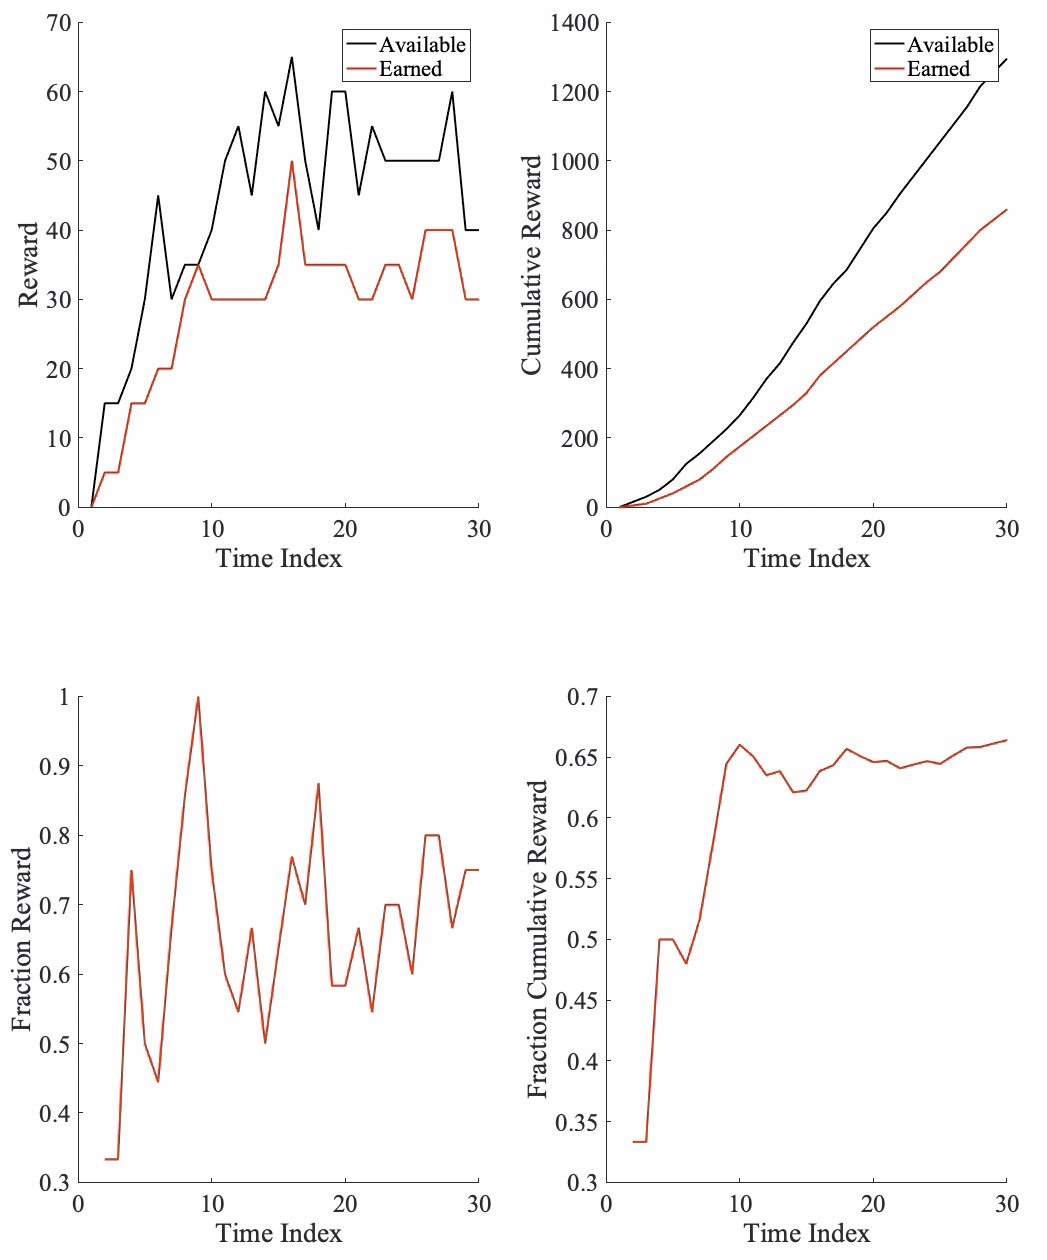
\includegraphics[width=3.4in]{rewards_earned.png}
    \caption{The left column shows the rewards earned per time step, where the left-top shows the rewards available and earned individually and the left-bottom shows the fractional rewards earned. The right column shows the accumulated rewards earned by the agents.}
    \label{fig:sim_rewards}
\end{figure}

\section{Conclusions}\label{sec:future}
In this paper, we present a distributed predictive task assignment algorithm for heterogeneous agents. 
We prove the algorithm's optimality-bound and demonstrate its effectiveness using simulations. 
We envisage this algorithm will see wide-spread use in many multi-agent and swarm applications. 
Future work will focus on incorporating multiple types of tasks, especially event-triggered tasks, and different kinds of heterogeneity.  


\section*{Acknowledgments}
This research was carried out at the Jet Propulsion Laboratory, California Institute of Technology, under a contract with the National Aeronautics and Space Administration. 
\copyright 2019 California Institute of Technology. All rights reserved.



{%\small
\bibliographystyle{IEEEtran}
\bibliography{main}
}
\ifextendedv
\begin{appendix}
\subsection{Proof of all theorems}
\begin{proof}[Proof of Lemma \ref{lemma:homogeneous_lp}]
The proof relies on showing that $\H(T^f,\A^f)$ can be transformed into a max-flow problem.
It should be noted first that the flow represents the motion of agents and the corresponding assignments to the values of $x,z$. We construct the directed \emph{flow graph} $G_\phi=(V_\phi,E_\phi)$  consisting of the following ingredients. For every vertex $j\in V$ and time step $\tau\in \K_k$ we add to $V_\phi$ two vertices denoted by $v_{j\tau},v'_{j\tau}$. We also add to $V_\phi$ the source and sink vertices $v_{\textup{source}}, v_{\textup{sink}}$. 

Let us describe the edges in $E_\phi$. For any $j\in V,\tau\in \K_k$ add the (directed) edge $(v_{j\tau}, v'_{j\tau})$, with cost equal to $-T^f_\tau[j]$, i.e., the negative value of the reward gained from accomplishing corresponding task, and assign the capacity of this edge to be $1$ (to ensure that the reward is collected only once). For any $j\in V,\tau\in \K_k$ we add another edge $(v_{j\tau}, v'_{j\tau})$, which is in parallel to the previously described edge: its cost is $0$ and its capacity is $\infty$. This ensures that agents that are chosen not to collect the reward associated with $T^f_\tau[j]$ will be able to progress to the next time step. Next, we add for any $j,j'$ such that $(j,j')\in \E$, and any $\tau\in \K_k$ the edge $(v'_{j\tau},v'_{j',\tau+1})$, with cost $0$ and capacity $\infty$ to mimic transitions of agents between different cells as time progresses. 
Finally, we connect the source and sink nodes. For every $j\in \V$ we add the edge $(v_{\textup{source}},v_{jk})$ with cost $0$ and capacity equal to number of agents from fleet $f$ whose initial location in time $k$ is $j$. We also add $(v_{j,k+K_{\textup{hor}}+1},v_{\textup{sink}})$ with zero cost infinite capacity. We set the incoming flow on $v_{\textup{source}}$ to be the size of $\A^f$. It is easy to verify that the optimal solution to the presented MCF is equal to the optimal solution of $\H(T^f,\A^f)$.
\end{proof}
\end{appendix}
\fi

\end{document}

%%% Local Variables:
%%% mode: latex
%%% TeX-master: t
%%% End:
